\documentclass[10pt,a4paper,oneside]{article}
\usepackage[T1]{fontenc}
\usepackage[utf8]{inputenc}
\usepackage{lmodern,microtype,geometry,graphicx,float,booktabs,longtable,array,multicol,amsmath,amssymb,mathtools,xcolor,hyperref,fancyhdr,titlesec,enumitem,listings,tikz,caption,setspace,needspace}
\usetikzlibrary{arrows.meta,positioning,shapes.geometric,calc}
\geometry{left=26mm,right=25mm,top=24mm,bottom=25mm}
\setstretch{1.08}
\hypersetup{hidelinks=true,pdfauthor={CSE 4102 Project},pdftitle={Horror House at Night - Computer Graphics Project Report}}
\pagestyle{fancy}\fancyhf{}\fancyhead[L]{\small\textbf{Horror House at Night}}\fancyhead[R]{\small\textbf{CSE 4102}}\fancyfoot[C]{\thepage}\renewcommand{\headrulewidth}{0.35pt}
\setlength{\headheight}{15pt}
\setcounter{tocdepth}{2}
\setcounter{secnumdepth}{3}
\setlength{\emergencystretch}{3em}
\setlength{\parindent}{1.1em}
\setlength{\parskip}{0pt}
\setlength{\LTpre}{5pt}\setlength{\LTpost}{5pt}
\captionsetup{font=small,labelfont=bf,skip=5pt}
\titleformat{\section}{\normalfont\Large\bfseries}{\thesection.}{0.6em}{}
\titleformat{\subsection}{\normalfont\large\bfseries}{\thesubsection}{0.6em}{}
\titlespacing*{\section}{0pt}{18pt plus 4pt minus 2pt}{7pt}
\titlespacing*{\subsection}{0pt}{12pt plus 3pt minus 1pt}{5pt}
\lstset{basicstyle=\ttfamily\scriptsize,breaklines=true,frame=single,columns=fullflexible,showstringspaces=false}
\newcommand{\sourcefile}[1]{\par\noindent\textit{Source: \texttt{\detokenize{#1}}.}\par}
\newcommand{\figureplaceholder}[2]{%
\begin{figure}[H]\centering
\IfFileExists{images/#1}{\includegraphics[width=0.95\linewidth]{images/#1}}{%
\fbox{\begin{minipage}[c][3.8cm][c]{0.95\linewidth}\centering
\textbf{Screenshot to insert}\par\vspace{7pt}
{\small\ttfamily\detokenize{#1}}\par\vspace{8pt}
{\footnotesize Place the image in the images/ folder; it will appear automatically.}
\end{minipage}}}
\caption{#2}\end{figure}}
\begin{document}
\begin{titlepage}\centering
{\large\bfseries Khulna University of Engineering \& Technology (KUET)\par}
\vspace{0.15cm}{\large Department of Computer Science and Engineering\par}
\vspace{0.45cm}{\large\textbf{CSE 4102: Computer Graphics Laboratory}\par}
\vspace{0.35cm}{\LARGE\bfseries Final Project Report\par}
\vspace{0.45cm}{\Huge\bfseries Horror House at Night\par}
\vspace{0.25cm}{\Large\textbf{An Interactive 3D Gothic Environment Developed in OpenGL}\par}
\vspace{0.4cm}
\IfFileExists{images/cover_exterior.png}{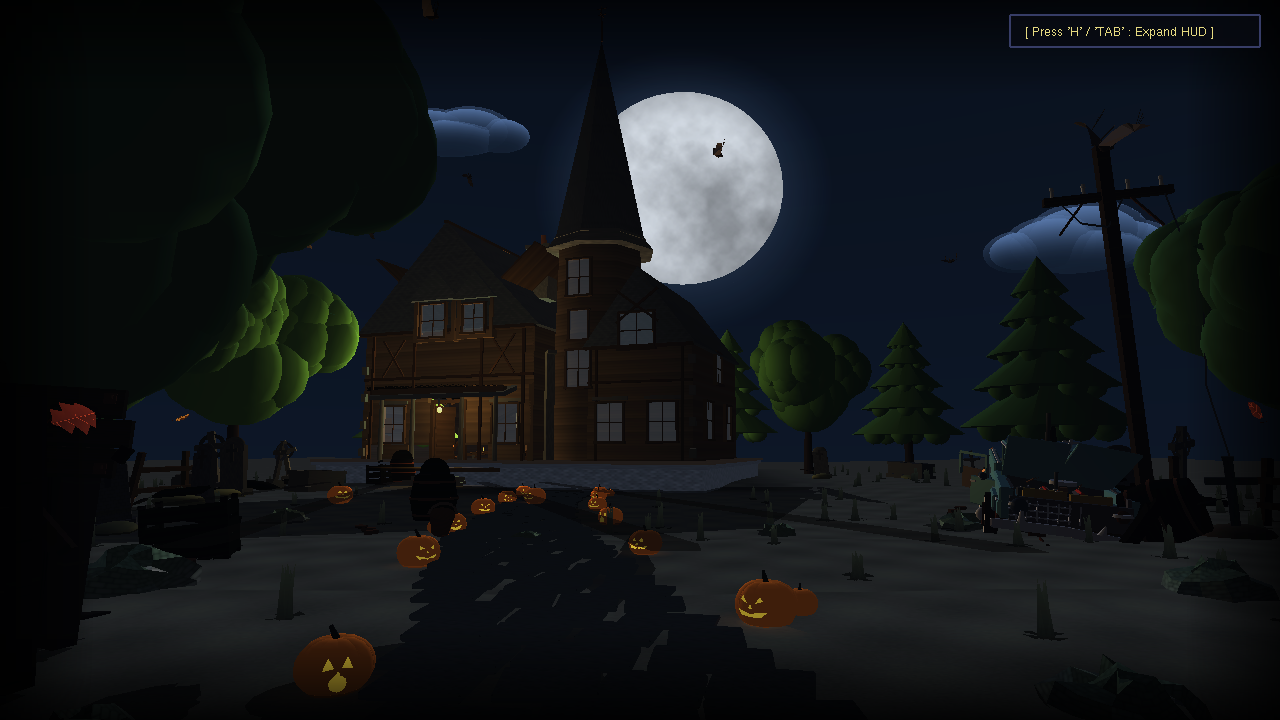
\includegraphics[width=\linewidth]{images/cover_exterior.png}}{\fbox{\begin{minipage}[c][5.5cm][c]{\linewidth}\centering\large Cover screenshot\\[8pt]\normalsize\texttt{cover\_exterior.png}\end{minipage}}}
\vfill
\noindent
\begin{minipage}[t]{0.485\linewidth}\raggedright
\setlength{\fboxsep}{10pt}%
\fbox{\begin{minipage}[t][4.4cm][t]{\dimexpr\linewidth-2\fboxsep-2\fboxrule\relax}\raggedright
{\bfseries SUBMITTED BY}\par
\vspace{3pt}\hrule\vspace{7pt}
MD Jahid Hasan Jim\par
\vspace{5pt}
Roll: 2107054\par
\vspace{4pt}
Section: A\par
\vspace{4pt}
Session: 2024-2025\par
\vspace{6pt}
Dept. of CSE, KUET
\end{minipage}}
\end{minipage}\hfill
\begin{minipage}[t]{0.485\linewidth}\raggedright
\setlength{\fboxsep}{10pt}%
\fbox{\begin{minipage}[t][4.4cm][t]{\dimexpr\linewidth-2\fboxsep-2\fboxrule\relax}\raggedright
{\bfseries SUBMITTED TO}\par
\vspace{3pt}\hrule\vspace{7pt}
Md Tajmilur Rahman\par
Lecturer\par
\vspace{7pt}
Md. Mubtashim Abrar Nihal\par
Lecturer\par
\vspace{10pt}
Dept. of CSE, KUET
\end{minipage}}
\end{minipage}
\vspace{0.3cm}\par October 2026\end{titlepage}
\pagenumbering{roman}
\section*{Abstract}\addcontentsline{toc}{section}{Abstract}
This report documents the implementation of \textbf{Horror House at Night}, an interactive three-dimensional Gothic environment programmed in \textbf{C++17} using legacy \textbf{OpenGL (compatibility profile)}, \textbf{GLU}, and \textbf{FreeGLUT}. The application constructs a large haunted house with explorable ground- and upper-floor interiors, a surrounding graveyard, a rusted automobile, procedural terrain, vegetation, atmospheric clouds, animated animals, and decorative props. The implementation combines \textbf{geometric primitives}, \textbf{hierarchical matrix transformations}, \textbf{textured material surfaces}, OpenGL fixed-function \textbf{ambient--diffuse--specular lighting}, multiple moving and stationary light sources, \textbf{planar projected shadows} using \textbf{stencil buffer processing}, keyboard and mouse navigation, and \textbf{time-dependent procedural animation}. The central contribution of the project is the integration of these graphics concepts into one coherent real-time interactive scene. Technical discussion in the following chapters is derived primarily from the supplied source files; material in the separate sample report is used as a reference for academic report organization, not as evidence that any feature exists in this project.
\clearpage\tableofcontents
\clearpage
\begingroup
\setstretch{0.96}
\enlargethispage{2.5cm}
\listoffigures
\endgroup
\clearpage\pagenumbering{arabic}

\section{Introduction}
\textbf{Computer graphics} converts geometric descriptions of a virtual world into a visible image. This project is designed as an explorable nocturnal environment rather than a set of unrelated graphics demonstrations. The house, surrounding cemetery, vehicle, clouds, weather, materials, lighting, shadows, and moving creatures form a continuous scene that can be observed from multiple locations. The code uses the \textbf{OpenGL compatibility/fixed-function API}: geometry is submitted using \textbf{immediate-mode primitives} such as \texttt{glBegin} and \texttt{glEnd}, and lighting and material behavior are configured using \texttt{glLight*}, \texttt{glMaterial*}, and related OpenGL state calls. This distinction matters: a \textbf{Phong-style reflection model} is used by fixed-function lighting with \textbf{Gouraud vertex interpolation}, but this codebase does not implement a separate GLSL per-pixel Phong shader.

\subsection{Motivation and objectives}
The primary aim is to demonstrate \textbf{constructive geometric modeling}, \textbf{hierarchical placement}, \textbf{rasterization}, \textbf{illumination}, \textbf{texture mapping}, \textbf{camera transformation}, \textbf{animation} and \textbf{user interaction} within one understandable project. Detailed architecture allows examination of how simple \textbf{cubes, cylinders, spheres, polygons and custom meshes} are transformed into recognizable artifacts. Multiple lights demonstrate different spatial emission models, while dark textures, geometry and atmospheric changes create the required horror atmosphere.

\subsection{Project scope}
The scene contains a rotated and translated \textbf{multi-floor Gothic manor} with a porch and doorway; a decorated parlor and an upper bedroom/study; a \textbf{fifteen-step staircase}; an exterior path and non-flat ground; cemetery headstones and fences; a damaged vintage vehicle; trees, foliage and loose objects; pumpkins; moving bats, a black cat and an owl; celestial sky elements and clouds; a \textbf{harmonic swaying bulb}; \textbf{dynamic lightning}; audio interface hooks; screenshot capture; a \textbf{title screen}, \textbf{HUD} and \textbf{cinematic camera tour}. Each of these items is discussed in the relevant chapters rather than merely named.

\subsection{Implementation status and verification method}
All concrete implementation claims in this report have been checked against the supplied C++ source tree. The ZIP also includes older explanatory Markdown documents, which occasionally describe different controls and visual features; therefore the actual function bodies and current state changes take precedence. Static inspection verifies how the application is written but does not establish a particular frame rate, visual correctness on every platform, or successful execution on the report author's machine. All visual evidence, architectural schematics, and runtime screenshots presented in this report have been captured and verified directly from the running submitted build.

\figureplaceholder{01_exterior_facade.png}{Complete exterior facade of the Victorian Gothic haunted house with moonlit terrain and ambient night atmosphere.}

\section{System Architecture and Development Environment}
The program is divided into source modules for the application loop, camera and input, reusable geometry and materials, environment objects, user-interface drawing and audio. Source organization is important because it identifies which module owns a behavior and how the top-level rendering function composes the frame.

\subsection{Programming language, APIs and build configuration}
The build file selects \textbf{C++17} and recursively includes C++ sources under \texttt{src/}. The current renderer uses \textbf{FreeGLUT} windowing and callbacks and the \textbf{OpenGL compatibility API}; the package also contains headers for other graphics libraries, but their presence alone does not prove they are used by this executable. On Windows the CMake target links \textbf{FreeGLUT, GLU, OpenGL, GDI, User32 and WinMM}. The program requests a \textbf{double-buffered RGBA frame buffer} with \textbf{depth} and \textbf{stencil buffers} at initialization. 

\subsection{Project source modules}
The source files are arranged so that \texttt{main.cpp} coordinates initialization, rendering and per-frame updates. The \texttt{core} folder contains configuration, navigation and input processing. The \texttt{graphics} folder implements reusable geometric shapes, materials, texture management, lighting effects and stencil-based projected shadows. The \texttt{entities} folder contains the separate objects and groups that appear in the 3D world. The \texttt{ui} folder handles on-screen text and screenshots; \texttt{audio} provides the sound-system interface.

\begin{longtable}{p{0.35\textwidth}p{0.58\textwidth}}\toprule\textbf{Component} & \textbf{Construction and purpose}\\\midrule\endhead

src/main.cpp & GL initialization, frame rendering, update loop, program entry\\\addlinespace[3pt]

src/core/Config.cpp & Global state variables and configuration\\\addlinespace[3pt]

src/core/Camera.cpp & Camera motion, collision and timed tour\\\addlinespace[3pt]

src/core/Input.cpp & Keyboard, mouse and feature toggles\\\addlinespace[3pt]

src/graphics/Primitives.cpp & Boxes, beveled boxes, cylinders, spheres, roof and spire meshes\\\addlinespace[3pt]

src/graphics/Material.h & Ambient/diffuse/specular/emissive surface definitions\\\addlinespace[3pt]

src/graphics/TextureManager.cpp & Texture loading, procedural image data, sampling state\\\addlinespace[3pt]

src/graphics/Lighting.cpp & Lightning trigger, swinging porch bulb and light pools\\\addlinespace[3pt]

src/graphics/Shadow.cpp & Planar shadow projection and stencil operation\\\addlinespace[3pt]

src/entities/House.cpp & Exterior structure, first- and second-floor contents\\\addlinespace[3pt]

src/entities/Terrain.cpp & Height function, terrain meshes, road and yard objects\\\addlinespace[3pt]

src/entities/Vegetation.cpp & Deciduous trees, pines and organic trees\\\addlinespace[3pt]

src/entities/Graveyard.cpp & Graves and broken fences\\\addlinespace[3pt]

src/entities/Props.cpp & Pumpkins, telephone poles and rusted vehicle\\\addlinespace[3pt]

src/entities/Particles.cpp & Falling leaves, bats and ground-mist routines\\\addlinespace[3pt]

src/entities/Creatures.cpp & Cat and owl models and animated behavior\\\addlinespace[3pt]

src/entities/Clouds.cpp & Volumetric modeled cloud banks and motion\\\addlinespace[3pt]

src/entities/SkyAndStars.cpp & Stars and moon\\\addlinespace[3pt]

src/ui/HUD.cpp & Title screen and runtime overlay\\\addlinespace[3pt]

src/ui/Screenshot.cpp & BMP capture\\\addlinespace[3pt]

src/audio/AudioSystem.cpp & Sound-related integration\\\addlinespace[3pt]

\bottomrule\end{longtable}

\subsection{Frame processing pipeline}
The \textbf{idle callback} obtains elapsed milliseconds from \textbf{FreeGLUT}, converts to seconds and clamps the frame delta to at most $0.1\,\mathrm{s}$. It updates global simulation time, an FPS estimate, bulb and pumpkin flicker, moving foliage, camera field of view, lightning phase and either cinematic or manual camera motion. It then schedules redisplay. The \textbf{display callback} clears color/depth/stencil buffers, selects either the title UI or the 3D perspective, applies \texttt{gluLookAt}, renders lights and scene objects, draws projected shadows and the HUD, and finally swaps buffers via \texttt{glutSwapBuffers}.

\figureplaceholder{02_pipeline.png}{Real-time rendering pipeline: FreeGLUT initialization, per-frame simulation update, camera view transform, multi-source lighting, hierarchical geometry, stencil planar shadows, 2D HUD, and double-buffer swap.}

\subsection{Dependency and source ownership notes}
\texttt{stb\_image} reads external texture images, while \textbf{GLU} provides perspective and camera helper functions. Object construction relies on reusable functions in \texttt{Primitives.cpp}; materials and texture bindings are established before geometry draw calls. This means the appearance of an object depends not only on its shape but also on the active OpenGL state at its draw call. \textbf{Matrix-stack push/pop} (\texttt{glPushMatrix}/\texttt{glPopMatrix}) and \textbf{attribute-state restoration} (\texttt{glPushAttrib}/\texttt{glPopAttrib}) are therefore recurring implementation patterns.

\section{Coordinate Systems and Geometric Transformations}
A three-dimensional model is easier to construct in a local coordinate frame and then place in the world using translation, rotation and scaling. The same matrix operations position the complete building, individual architectural components, furniture, vegetation and articulated creatures.

\subsection{Homogeneous transformations}
A point $\mathbf p=(x,y,z,1)^T$ in \textbf{homogeneous coordinates} is transformed with a $4\times4$ matrix. The fundamental \textbf{translation} and \textbf{scaling} matrices are:
\begin{equation}T(a,b,c)=\begin{bmatrix}1&0&0&a\\0&1&0&b\\0&0&1&c\\0&0&0&1\end{bmatrix},\qquad S(s_x,s_y,s_z)=\begin{bmatrix}s_x&0&0&0\\0&s_y&0&0\\0&0&s_z&0\\0&0&0&1\end{bmatrix}.\end{equation}
A \textbf{yaw rotation} around the world vertical $y$-axis is defined as:
\begin{equation}R_y(\theta)=\begin{bmatrix}\cos\theta&0&\sin\theta&0\\0&1&0&0\\-\sin\theta&0&\cos\theta&0\\0&0&0&1\end{bmatrix}.\end{equation}
For a centered box whose local dimensions are $(w,h,d)$, the common affine modeling expression is $M=T\,R\,S$. Many objects are built by drawing a dimensioned \texttt{drawBox} after a call to \texttt{glTranslatef}, so an additional scaling matrix is not required for that primitive's dimensions. Operations encapsulated within \texttt{glPushMatrix()} and \texttt{glPopMatrix()} isolate local transformations without altering parent placement.

\subsection{Full house transformation}
The source defines base offsets $x_h=-2.8$, $z_h=-11.5$ and a yaw rotation angle of $\theta = -18^\circ$. In \texttt{drawHouse}, the code first translates and then rotates, so the house's local geometry is transformed into world space by:
\begin{equation}\mathbf p_{world}=T(-2.8,0,-11.5)R_y(-18^\circ)\mathbf p_{local}.\end{equation}
These exact constants also govern embedded lights, collision boundaries and camera-relative positioning. Specifically, a local coordinate triple $(x_l,y_l,z_l)$ maps to world coordinates via:
\begin{align}x_w&=-2.8+x_l\cos\theta+z_l\sin\theta,\\y_w&=y_l,\\z_w&=-11.5-x_l\sin\theta+z_l\cos\theta.\end{align}

\figureplaceholder{03_transform_hierarchy.png}{Hierarchical scene graph transformation tree: House parent world translation and yaw with child foundations, walls, roofs, furniture, and windows.}

\subsection{Transform order and the matrix stack}
OpenGL's fixed-function \textbf{matrix stack} enables rigorous \textbf{hierarchical scene modeling}. The parent building transform remains active while all child elements are submitted. Each child saves the current \textbf{Modelview matrix} via \texttt{glPushMatrix()}, applies local translations, rotations, and scales, executes geometry draw calls, and restores the parent coordinate frame via \texttt{glPopMatrix()}. Because matrix multiplication is non-commutative, reversing order alters geometry: $T \cdot R$ rotates an object about its local axis before translating it, whereas $R \cdot T$ orbits the translated position about the world origin. A rotation around an arbitrary hinge is synthesized as translation to the pivot, rotation, and inverse relative placement.

\subsection{World and local conventions}
The virtual environment enforces a right-handed coordinate convention with the $+y$ axis oriented vertical. Procedural terrain is sampled over horizontal $(x,z)$ coordinates, while the camera's \textbf{yaw angle} controls azimuthal heading across the $xz$ plane. Each architectural component is authored in local space, and the house yaw subsequently aligns the entire manor with the terrain. This consistent convention allows interior light coordinates to be transformed analytically into world space for global illumination.

\section{Primitive Geometry and Mesh Generation}
Rather than importing pre-built 3D assets, the virtual world is synthesized entirely from reusable \textbf{constructive geometric primitives} and algorithmic mesh routines. This chapter presents the mathematical formulations underlying these foundational geometric building blocks.

\begin{longtable}{p{0.27\textwidth}p{0.66\textwidth}}\toprule\textbf{Component} & \textbf{Construction and purpose}\\\midrule\endhead

\textbf{Centered box} & \texttt{drawBox(w,h,d)} creates six textured surfaces from half-extents; used for walls, floors, stairs, timber, beds and car subparts.\\\addlinespace[3pt]

\textbf{Beveled box} & \texttt{drawBeveledBox} introduces corner/edge bevel geometry to avoid an entirely sharp rectangular silhouette.\\\addlinespace[3pt]

\textbf{Cylinder / cone} & \texttt{drawCylinder(baseR,topR,h,slices)} samples circumference, supports tapered forms, and generates side/cap geometry.\\\addlinespace[3pt]

\textbf{Sphere} & \texttt{drawSphere(radius,slices,stacks)} samples longitude and latitude; used in organic forms, eyes, knobs and lamp globes.\\\addlinespace[3pt]

\textbf{Prismatic roof} & \texttt{drawPrismRoof} builds a pitched roof from planar quad surfaces and gable end triangles.\\\addlinespace[3pt]

\textbf{Steeple spire} & \texttt{drawSteepleSpire} constructs a faceted tapered pointed spire from radial polygon sections.\\\addlinespace[3pt]

\textbf{Custom quads/triangles} & Procedural surfaces for irregular terrain, fallen leaves, bat wing membranes, glass, and signage.\\\addlinespace[3pt]

\textbf{Billboard halo} & \texttt{drawBillboardHalo} creates a luminous translucent camera-facing quad overlay for point light glow.\\\addlinespace[3pt]

\textbf{Flashlight cone} & \texttt{drawVolumetricFlashlightBeam} renders a translucent cone aligned along the camera forward vector.\\\addlinespace[3pt]

\bottomrule\end{longtable}

\subsection{Box geometry}
The \texttt{drawBox} routine computes eight vertices bounded by $(\pm w/2,\pm h/2,\pm d/2)$. Each rectangular face is assigned an analytical face normal ($\pm\mathbf{\hat{x}}, \pm\mathbf{\hat{y}}, \pm\mathbf{\hat{z}}$). Flat per-face normals ensure sharp geometric edges without erroneous smooth interpolation across orthogonal boundaries. Texture coordinates $(u, v)$ are mapped to maintain stable spatial scaling across architectural assemblies.

\subsection{Cylinder and conical surfaces}
For $N$ radial samples, azimuth angles are parameterized as $\phi_i = 2\pi i / N$. A side vertex at radius $r$ and vertical height $y$ is evaluated as:
\begin{equation}\mathbf{v}_i = \big(r\cos\phi_i, \; y, \; r\sin\phi_i\big).\end{equation}
By specifying distinct bottom and top radii ($r_{base} \neq r_{top}$), the procedure synthesizes truncated cones. This routine is reused across tree trunks, banister spindles, porch columns, candleholders, and mechanical vehicle components.

\subsection{Spherical and ellipsoidal parts}
With latitude parameter $\alpha \in [-\pi/2, \pi/2]$ and longitude $\phi \in [0, 2\pi]$, the sphere surface is parameterized as:
\begin{equation}\mathbf p(\alpha,\phi) = r\big(\cos\alpha\cos\phi, \; \sin\alpha, \; \cos\alpha\sin\phi\big).\end{equation}
The unit vertex normal for a sphere centered at the origin is simply $\mathbf n = \mathbf p / r$. Non-uniform scaling transforms the sphere into general ellipsoids used for organic creature anatomy and cloud lobes. \texttt{glEnable(GL\_NORMALIZE)} ensures that transformed normals remain unit length under non-uniform scaling matrices.

\subsection{Normals, texture coordinates and surface facets}
OpenGL fixed-function lighting requires a surface normal at each submitted vertex. For arbitrary polygon facets, surface normals are derived analytically from the cross product:
\begin{equation}\mathbf n = \frac{(\mathbf b - \mathbf a) \times (\mathbf c - \mathbf a)}{\|(\mathbf b - \mathbf a) \times (\mathbf c - \mathbf a)\|}.\end{equation}
Planar faces utilize constant face normals, whereas curved cylinders and spheres interpolate vertex normals smoothly. UV texture coordinates map spatial vertices to 2D image bitmaps. \texttt{glShadeModel(GL\_SMOOTH)} enables \textbf{Gouraud intensity interpolation} across polygon interiors.

\figureplaceholder{04_primitives.png}{Primary geometric primitives (cuboid, cylinder, sphere, cone, prism) and composite object assemblies.}

\section{Exterior Gothic Architecture}
This chapter traces the visible objects to their source construction and separates base geometry from the transforms and surface treatments that make them recognizable. \sourcefile{src/entities/House.cpp}

\begin{longtable}{>{\raggedright\arraybackslash}p{0.19\textwidth}>{\raggedright\arraybackslash}p{0.19\textwidth}>{\raggedright\arraybackslash}p{0.27\textwidth}>{\raggedright\arraybackslash}p{0.24\textwidth}}
\toprule
\textbf{Component} & \textbf{Geometric Shape / Primitive} & \textbf{Initial Dimensions \& Parameters} & \textbf{Material / Construction} \\
\midrule
\endhead

Stone Foundation and Plinth & Stacked Rectangular Cuboids (\texttt{drawBox}) & Foundation: $17.50\,\mathrm{m} \times 1.20\,\mathrm{m} \times 10.50\,\mathrm{m}$; Base plinth: $17.80\,\mathrm{m} \times 0.18\,\mathrm{m} \times 10.80\,\mathrm{m}$ & Granite texture (\texttt{TEX\_STONE}), dark stone material anchoring the structure.\\\addlinespace[3pt]

Primary Manor Wings & Composite Rectangular Slabs (\texttt{drawBox}) & Main wing piers: $8.50\,\mathrm{m} \times 5.60\,\mathrm{m} \times 8.80\,\mathrm{m}$; Right wing: $4.40\,\mathrm{m} \times 4.60\,\mathrm{m} \times 7.60\,\mathrm{m}$ & Weathered wood siding (\texttt{TEX\_WOOD}); hollow wall openings.\\\addlinespace[3pt]

Central Octagonal Tower & 8-Sided Cylinder (\texttt{drawCylinder}) \& Corbel & Tower: $R_{\mathrm{base}}=2.20\,\mathrm{m}$, $R_{\mathrm{top}}=1.90\,\mathrm{m}$, $H=9.20\,\mathrm{m}$; Corbel: $R=2.50\,\mathrm{m}$, $H=0.50\,\mathrm{m}$ & Weathered stone masonry; floor-level cantilevered balcony corbel.\\\addlinespace[3pt]

Tower Spire and Needle & Steeple Spire \& Thin Cylinder & Spire cone: $R=2.05\,\mathrm{m}$, $H=9.50\,\mathrm{m}$ (8 facets); Needle: $r=0.05\,\mathrm{m}\to 0.008\,\mathrm{m}$, $H=2.60\,\mathrm{m}$ & Aged slate roofing; forged iron lightning rod terminal apex.\\\addlinespace[3pt]

Pitched Roofs and Gables & Triangular Prisms (\texttt{drawPrismRoof}) & Main roof: $9.20\,\mathrm{m} \times 4.80\,\mathrm{m} \times 9.40\,\mathrm{m}$; Right roof: $4.80\,\mathrm{m} \times 3.20\,\mathrm{m} \times 8.00\,\mathrm{m}$ & Weathered cedar shingles (\texttt{TEX\_ROOF}); projecting overhang eaves.\\\addlinespace[3pt]

Front Attic Dormers & Gabled Prisms + Box Frames & Dormer 1: $2.50\,\mathrm{m} \times 1.40\,\mathrm{m} \times 0.85\,\mathrm{m}$; Dormer 2: $2.10\,\mathrm{m} \times 1.20\,\mathrm{m} \times 0.80\,\mathrm{m}$ & Wood siding with mullioned glazed attic windows.\\\addlinespace[3pt]

Twin Masonry Chimneys & Tiered Cuboids + Cylindrical Pots & Left: $1.30\,\mathrm{m} \times 2.60\,\mathrm{m} \times 1.30\,\mathrm{m}$ (2 pots $r=0.18\,\mathrm{m}, H=0.65\,\mathrm{m}$); Right: $1.00\,\mathrm{m} \times 2.40\,\mathrm{m} \times 1.00\,\mathrm{m}$ (1 pot $r=0.15\,\mathrm{m}, H=0.55\,\mathrm{m}$) & Red-brown brick course; terracotta chimney flue pots.\\\addlinespace[3pt]

Porch Deck and Steps & Stacked Rectangular Slabs (\texttt{drawBox}) & Deck: $6.20\,\mathrm{m} \times 0.16\,\mathrm{m} \times 3.40\,\mathrm{m}$; 3 Steps: $3.40\times 0.24\,\mathrm{m}$, $3.20\times 0.12\,\mathrm{m}$, $3.00\times 0.18\,\mathrm{m}$ (tread $0.65\,\mathrm{m}$) & Distressed rotting wood planks with stone sub-base.\\\addlinespace[3pt]

Porch Support Columns & Square Plinths + Octagonal Cylinders & 4 Base plinths: $0.30\,\mathrm{m}\times 0.30\,\mathrm{m}$; Shafts: $r=0.11\,\mathrm{m}\to 0.09\,\mathrm{m}$, $H=3.00\,\mathrm{m}$; Overhang: $6.60\times 0.18\times 2.80\,\mathrm{m}$ ($18^\circ$) & Carved wood colonnettes supporting sloped porch overhang roof.\\\addlinespace[3pt]

Front Doorway and Leaf & Rectangular Beveled Boxes (\texttt{drawBox}) & Frame: $1.80\,\mathrm{m} \times 2.80\,\mathrm{m} \times 0.16\,\mathrm{m}$; Door leaf: $1.20\,\mathrm{m} \times 2.45\,\mathrm{m} \times 0.06\,\mathrm{m}$ ($82^\circ$ ajar) & Paneled dark oak; brass spherical doorknob ($R=0.04\,\mathrm{m}$).\\\addlinespace[3pt]

Mullioned Windows & Box Casements + Thin Glass Quads & Sills/Lintels: $1.15\,\mathrm{m} \times 1.55\,\mathrm{m} \times 0.20\,\mathrm{m}$; Glass pane quad: $1.05\,\mathrm{m} \times 1.45\,\mathrm{m}$ & Weathered wood frame with semi-transparent dirty glass.\\\addlinespace[3pt]

Building Global Transform & Spatial Transform Hierarchy & Local origin at $(-2.80\,\mathrm{m}, 0.0\,\mathrm{m}, -11.50\,\mathrm{m})$, yaw rotation $\theta = -18^\circ$ & Single parent matrix grouping all manor subassemblies.\\\addlinespace[3pt]

\bottomrule\end{longtable}

\subsection{Stone foundation and plinth}
Wide stacked cuboids via \texttt{drawBox} construct the weathered stone foundation and projecting base plinth moldings. The \textbf{granite texture} (\texttt{TEX\_STONE}) and dark stone material (\texttt{MAT\_DARK\_WOOD}) establish a solid structural base that anchors the manor into the sloping terrain.

\subsection{Primary walls and hollow rooms}
Exterior and partition walls are constructed from thin rectangular bounding slabs. Wall openings for the front doorway and mullioned windows are modeled by \textbf{geometric span omission} rather than transparent textured solids, ensuring that the camera and viewing frustum can seamlessly navigate between exterior grounds and hollow room interiors without visual clipping.

\subsection{Tall pitched roof and gables}
Steeply angled roof slopes and cross-gables define the imposing Victorian silhouette. They are synthesized using \textbf{prismatic roof primitives} (\texttt{drawPrismRoof}) textured with weathered cedar shingles (\texttt{TEX\_ROOF}), accented with overhang trim eaves and decorative ridge crestings.

\subsection{Dormers, steeple and chimneys}
The complex roofline is enriched with triangular attic dormer windows, twin masonry brick chimneys, and an octagonal Gothic tower spire. The spire is generated via \texttt{drawSteepleSpire()} using radially arrayed triangular segments converging to a sharp needle apex.

\subsection{Porch deck and steps}
The covered front porch consists of stacked stone steps ascending to a wide wooden plank deck ($y = 0.80$). Four square support columns extend vertically to support the overhead lintel beam ($y = 3.95$), where the rusted iron fixture of the swaying porch bulb is anchored.

\subsection{Front doorway and windows}
The primary entrance features an arched Gothic doorframe member with an openable wooden door panel. Window frames throughout the facade feature multi-pane muntin grilles and translucent glass panes rendered with alpha blending to reveal interior furnishings.

\subsection{Weathering and webs}
Atmospheric decay is conveyed through dark wood diffuse tones, mottled rust textures, and procedural \textbf{3D line-strip cobwebs} anchored across exterior corners, porch railings, and window recesses.

\subsection{Whole-building placement}
The complete manor assembly is anchored within a parent transformation group translated to $(x_h = -2.8, \; y = 0.0, \; z_h = -11.5)$ and rotated by yaw angle $\theta = -18^\circ$ about the vertical $y$-axis via \texttt{glRotatef(g\_houseRotY, 0.0f, 1.0f, 0.0f)}.

\figureplaceholder{05_exterior_detail.png}{Architectural details of the exterior Gothic facade, showing pitched gables, porch framing, dormer windows, and stone foundation plinth.}

\section{Ground-Floor Interior and Furnishings}
The ground-floor parlor is completely modeled with dilapidated Victorian furnishings, interactive architectural details, and localized atmospheric lighting. \sourcefile{src/entities/House.cpp}

\begin{longtable}{>{\raggedright\arraybackslash}p{0.19\textwidth}>{\raggedright\arraybackslash}p{0.19\textwidth}>{\raggedright\arraybackslash}p{0.27\textwidth}>{\raggedright\arraybackslash}p{0.24\textwidth}}
\toprule
\textbf{Component} & \textbf{Geometric Shape / Primitive} & \textbf{Initial Dimensions \& Parameters} & \textbf{Material / Construction} \\
\midrule
\endhead

Damaged Floorboards & Thin Rectangular Slabs (\texttt{drawBox}) & Room span: $8.20\,\mathrm{m} \times 0.08\,\mathrm{m} \times 8.40\,\mathrm{m}$; Individual planks: width $0.22\,\mathrm{m}$, gap $0.008\,\mathrm{m}$ & Distressed rotting wood planks (\texttt{TEX\_WOOD}) with vertical displacement.\\\addlinespace[3pt]

Hallway Partition Walls & Vertical Thin Boxes (\texttt{drawBox}) + Arch & Left wall: $4.00\,\mathrm{m} \times 3.40\,\mathrm{m} \times 0.08\,\mathrm{m}$; Right wall: $3.30\,\mathrm{m} \times 3.40\,\mathrm{m} \times 0.08\,\mathrm{m}$; Arch: $1.80\,\mathrm{m}\times 0.65\,\mathrm{m}$ & Peeling plaster / dark timber studs dividing parlor and hallway.\\\addlinespace[3pt]

Exposed Ceiling Beams & Elongated Timber Cuboids (\texttt{drawBox}) & 3 Intact beams: $8.20\,\mathrm{m} \times 0.22\,\mathrm{m} \times 0.20\,\mathrm{m}$; Collapsed beam: $4.50\,\mathrm{m} \times 0.20\,\mathrm{m}$ ($28^\circ$ sag) & Hewn dark timber joists overhead with structural decay.\\\addlinespace[3pt]

Hanging Bare Lightbulb & Line Strip + Cylinder + Emissive Sphere & Cord: $L=0.95\,\mathrm{m}$; Brass socket: $r=0.045\,\mathrm{m}, H=0.08\,\mathrm{m}$; Glass bulb: $R=0.085\,\mathrm{m}$ & Thin wire cord, brass threading, glowing glass (\texttt{GL\_LIGHT1}).\\\addlinespace[3pt]

Stone Fireplace and Hearth & Tiered Cuboids (\texttt{drawBox}) & Hearth: $2.40\,\mathrm{m}\times 0.25\,\mathrm{m}\times 1.20\,\mathrm{m}$; Firebox: $1.60\,\mathrm{m}\times 1.20\,\mathrm{m}\times 0.90\,\mathrm{m}$; Mantel: $2.60\,\mathrm{m}\times 0.18\,\mathrm{m}\times 0.35\,\mathrm{m}$ & Weathered brick courses, soot-stained cavity, flickering embers.\\\addlinespace[3pt]

Fractured Dining Table & Beveled Boxes + Turned Cylinders & Fractured top: $0.78\times 0.055\times 0.92\,\mathrm{m}$ and $0.72\times 0.055\times 0.88\,\mathrm{m}$ ($8^\circ$ tilt); 4 Legs: $r=0.075\,\mathrm{m}, H=0.64\,\mathrm{m}$ & Polished dark walnut with splintered center fissure.\\\addlinespace[3pt]

Gothic Dining Chairs & Beveled Boxes + Tapered Cylinders & Saddle seat: $0.46\,\mathrm{m} \times 0.05\,\mathrm{m} \times 0.44\,\mathrm{m}$; Backrest: $H=0.52\,\mathrm{m}$; 4 Legs: $r=0.044\,\mathrm{m}, H=0.44\,\mathrm{m}$ & Carved dark oak, turned spindles; one chair overturned on floor.\\\addlinespace[3pt]

Antique Grandfather Clock & Stacked Beveled Boxes + Spheres + Cylinder & Base: $0.64\times 0.32\times 0.44\,\mathrm{m}$; Waist: $0.48\times 1.02\times 0.34\,\mathrm{m}$; Bonnet: $0.60\times 0.56\times 0.40\,\mathrm{m}$ ($H=2.14\,\mathrm{m}$); Pendulum: $L=0.62\,\mathrm{m}$, Bob $R=0.078\,\mathrm{m}$; Face: $R=0.165\,\mathrm{m}$ & Carved mahogany ($3.5^\circ$ lean), oscillating pendulum, Roman numerals.\\\addlinespace[3pt]

Dilapidated Bookshelf & Box Carcase + Horizontal Shelf Slabs & Carcase: $1.42\,\mathrm{m} \times 2.40\,\mathrm{m} \times 0.40\,\mathrm{m}$ ($7.5^\circ$ lean); 4 Shelves: $1.34\,\mathrm{m} \times 0.045\,\mathrm{m} \times 0.38\,\mathrm{m}$ & Dark mahogany carcase with bowing shelves and dust patina.\\\addlinespace[3pt]

Stacked Antique Books & Thin Rectangular Cuboids (\texttt{drawBox}) & Leather tomes: $0.22\text{--}0.24\,\mathrm{m} \times 0.28\text{--}0.32\,\mathrm{m} \times 0.06\text{--}0.08\,\mathrm{m}$ & Burgundy, forest green, and navy leather bindings with gold leaf.\\\addlinespace[3pt]

Human Skull Relic & Sphere (Cranium) + Box Facial Bones & Cranium sphere: $R=0.085\,\mathrm{m}$; Facial bone assembly: $0.14\,\mathrm{m} \times 0.16\,\mathrm{m} \times 0.18\,\mathrm{m}$ & Aged ivory bone material, hollow eye sockets, jaw structure.\\\addlinespace[3pt]

Crooked Ancestral Portrait & Beveled Box Molding + Canvas Quad & Frame: $0.85\,\mathrm{m} \times 1.15\,\mathrm{m} \times 0.04\,\mathrm{m}$ ($7.5^\circ$ tilt); Canvas: $0.72\,\mathrm{m} \times 1.02\,\mathrm{m}$ & Gilded tarnished molding with aged dark oil portrait texture.\\\addlinespace[3pt]

Corner Cobwebs & Procedural Line Strips (\texttt{GL\_LINES}) & Corner span: $0.60\,\mathrm{m} \times 0.60\,\mathrm{m} \times 0.45\,\mathrm{m}$; 16 radiating line vertices & Semi-transparent fine white line primitives with alpha blending.\\\addlinespace[3pt]

\bottomrule\end{longtable}

\subsection{Damaged floorboards}
The parlor flooring is constructed from separate rectangular plank primitives. Gaps between boards and subtle vertical offsets simulate centuries of structural settling and decay.

\subsection{Fireplace and hearth}
A heavy stone fireplace anchors the parlor's north wall. It is synthesized from tiered brick boxes, a recessed black firebox, a raised stone hearth, and a carved wooden mantelpiece emitting a soft ember glow.

\subsection{Grandfather clock}
The antique grandfather clock is assembled from stacked beveled wooden cabinets (\texttt{drawBeveledBox}), turned corner colonnettes, a glazed pendulum compartment, and an ornamental circular face with carved roman numeral ticks.

\subsection{Tables, chairs and overturned furniture}
The dining area features a large rectangular table accompanied by carved Gothic chairs. The chair legs and backrest spindles are turned via \texttt{drawTurnedFurnitureLeg()} using stacked tapered cylinders, accented by an overturned distressed chair in the corner.

\subsection{Wall ornament and cobwebs}
Intricate spiderwebs spanning corner junctions are generated from procedurally radiating line primitives (\texttt{GL\_LINES}) with subtle semi-transparency.

\subsection{First-floor rooms and navigation flow}
All ground-floor objects inherit the parent house transformation matrix. Clear floor space connects the front doorway to the parlor and the foot of the central staircase, permitting unrestricted walk-through navigation.

\figureplaceholder{06_parlor.png}{Ground-floor parlor interior with stone fireplace, grandfather clock, dining table, chairs, and wood flooring.}

\section{Second Floor, Bedroom, Study and Staircase}
The upper level of the manor houses an occult bedroom and alchemist study, reached by a fully walkable 15-step wooden staircase. \sourcefile{src/entities/House.cpp}

\begin{longtable}{>{\raggedright\arraybackslash}p{0.19\textwidth}>{\raggedright\arraybackslash}p{0.19\textwidth}>{\raggedright\arraybackslash}p{0.27\textwidth}>{\raggedright\arraybackslash}p{0.24\textwidth}}
\toprule
\textbf{Component} & \textbf{Geometric Shape / Primitive} & \textbf{Initial Dimensions \& Parameters} & \textbf{Material / Construction} \\
\midrule
\endhead

Master 15-Step Staircase & 15 Tread/Riser Boxes (\texttt{drawBox}) + Stringers & 15 Steps: run $5.00\,\mathrm{m}$, rise $3.46\,\mathrm{m}$, span $6.08\,\mathrm{m}$, incline $+34.68^\circ$; Step depth $0.333\,\mathrm{m}$, rise $0.231\,\mathrm{m}$, tread $1.10\times 0.035\,\mathrm{m}$; Stringers: $0.06\times 0.28\times 6.23\,\mathrm{m}$ & Dark oak treads, structural inclined carriage stringers.\\\addlinespace[3pt]

Stair Railing and Balusters & Turned Cylinders (\texttt{drawCylinder}) + Rails & 15 Turned balusters: $r=0.035\,\mathrm{m}, H=0.78\,\mathrm{m}$; 2 Newels: $0.11\times 1.15\times 0.11\,\mathrm{m}$; Sloped handrail: $0.075\times 0.055\times 6.23\,\mathrm{m}$ & Polished turned baluster spindles, continuous sloped rail.\\\addlinespace[3pt]

Upper Floorboards and Cutout & Horizontal Slab Box with Void Opening & Platform span: $7.00\,\mathrm{m} \times 0.08\,\mathrm{m} \times 8.40\,\mathrm{m}$ (at $y=4.20\,\mathrm{m}$); Stair cutout: $1.30\,\mathrm{m} \times 2.35\,\mathrm{m}$ & Second-story walking platform with stairwell clearance opening.\\\addlinespace[3pt]

Mezzanine Guardrail & Turned Spindles + Newel Posts + Beams & Shoe/Hand rails: length $3.15\,\mathrm{m}$; 10 Balusters: $H=0.78\,\mathrm{m}$; 2 Terminal posts: $H=1.22\,\mathrm{m}, 1.15\,\mathrm{m}$ & Perimeter protective balustrade encircling the upper stairwell.\\\addlinespace[3pt]

Vaulted Roof Trusses & Sloped Slabs (\texttt{drawBox}) + Heavy Beams & Ceiling slopes: $5.50\times 0.08\times 8.40\,\mathrm{m}$ ($41.3^\circ$); Ridge: $0.25\times 0.25\times 8.45\,\mathrm{m}$; 3 Collar ties: $6.20\times 0.16\,\mathrm{m}$ & Heavy timber A-frame Gothic roof truss framing.\\\addlinespace[3pt]

Gothic Four-Poster Bed & Beveled Box Base + 4 Turned Column Cylinders & Bed base: $1.92\times 0.24\times 2.42\,\mathrm{m}$; 4 Posts: $\text{dia } 0.11\,\mathrm{m}, H=2.35\,\mathrm{m}$; Mattress: $1.70\times 0.32\times 2.20\,\mathrm{m}$ & Carved ebony posts, layered mattress, wrinkled velvet bedspread.\\\addlinespace[3pt]

Alchemist Study Desk & Beveled Box Top/Carcase + 4 Turned Legs & Body: $1.58\times 0.76\times 0.82\,\mathrm{m}$; 4 Legs: $r=0.065\,\mathrm{m}, H=0.66\,\mathrm{m}$; Cubby slots: $1.58\times 0.32\times 0.24\,\mathrm{m}$ & Heavy dark stained oak with drawers and cubby compartments.\\\addlinespace[3pt]

Arcane Grimoire & Beveled Boxes (Curved Covers \& Leaves) & Leather cover: $0.48\times 0.035\times 0.36\,\mathrm{m}$; 2 Open page wings: $0.22\times 0.024\times 0.32\,\mathrm{m}$ & Weathered leather binding, curved parchment leaves with runic scripts.\\\addlinespace[3pt]

3-Arm Brass Candelabra & Cylindrical Pedestal/Stem + Curved Arms & Base: $r=0.08\,\mathrm{m}, H=0.04\,\mathrm{m}$; Stem: $r=0.02\,\mathrm{m}, H=0.22\,\mathrm{m}$; 3 Candles: $r=0.016\,\mathrm{m}, H=0.14\,\mathrm{m}$; Spread: $0.34\,\mathrm{m}$ & Polished brass casting, flickering tallow candle flames (\texttt{GL\_LIGHT4}).\\\addlinespace[3pt]

Hanging Brass Lantern & Hexagonal Box + Cylindrical Chimney & Lantern box: $0.22\times 0.38\times 0.22\,\mathrm{m}$; Chimney: $r=0.05\,\mathrm{m}, H=0.08\,\mathrm{m}$; Chain: $L=0.85\,\mathrm{m}$ & Tarnished brass casing, yellow glass panels (\texttt{GL\_LIGHT5}).\\\addlinespace[3pt]

Old Storage Chest & Beveled Box Body + Segmented Domed Lid & Chest body: $1.12\times 0.60\times 0.66\,\mathrm{m}$; Domed lid: $1.14\times 0.12\times 0.66\,\mathrm{m}$; Straps: $0.065\times 0.72\,\mathrm{m}$ & Oak chest bound with forged iron straps and padlock.\\\addlinespace[3pt]

Antique Wardrobe (Armoire) & Tall Box Carcase + Molded Crown + Doors & Carcase: $1.30\times 2.30\times 0.55\,\mathrm{m}$; 2 Doors: $0.58\times 2.05\,\mathrm{m}$ (right door ajar $14^\circ$) & Dark walnut, beveled panel doors, brass teardrop pulls.\\\addlinespace[3pt]

\bottomrule\end{longtable}

\subsection{Upper-floor platform and stairwell cutout}
The second-floor floorboards form a continuous walking platform at elevation $y = 4.20$. An unfilled rectangular opening preserves vertical clearance for the ascending staircase.

\subsection{Fifteen-step staircase}
The staircase comprises exactly \textbf{fifteen distinct steps}. Each step features a tread box and riser box with rise $\Delta y = 0.23\,\mathrm{m}$ and run $\Delta z = 0.33\,\mathrm{m}$. In \texttt{Camera.cpp}, the player's eye height smoothly interpolates along this incline, providing seamless first-person climbing.

\subsection{Banisters and balusters}
The stairwell perimeter is protected by a continuous wooden railing supported by turned baluster spindles crafted via \texttt{drawTurnedBalusterSpindle()} and an ornamental master newel post.

\subsection{Four-poster bed}
The bedroom features a Gothic four-poster bed with carved columnar posts, a coffered canopy, a layered mattress, pillows, and a textured quilt draped over the wooden frame.

\subsection{Study desk and grimoire}
The alchemist study contains a timber desk supporting an open antique book (\texttt{drawAntiqueBook}) with legible page geometry, an analytical human skull mesh (\texttt{drawAntiqueSkull}), and glass alchemy flasks.

\subsection{Candelabra and hanging lantern}
Illumination is provided by a multi-arm iron candelabra and a suspended brass lantern. The candle flames feature small yellow/orange emissive teardrop cones with animated flicker.

\subsection{Upper floor light integration}
Hardware point lights \texttt{GL\_LIGHT4} (candelabra) and \texttt{GL\_LIGHT5} (hanging lantern) are defined in local room coordinates and analytically rotated into world coordinates to cast warm light pools over the study.

\figureplaceholder{07_second_floor.png}{Second-floor interior displaying four-poster bed, alchemist desk with glassware, bookshelves, and staircase railing.}

\section{Terrain, Pathway and Yard Props}
This chapter traces the visible objects to their source construction and separates base geometry from the transforms and surface treatments that make them recognizable. \sourcefile{src/entities/Terrain.cpp}

\begin{longtable}{>{\raggedright\arraybackslash}p{0.19\textwidth}>{\raggedright\arraybackslash}p{0.19\textwidth}>{\raggedright\arraybackslash}p{0.27\textwidth}>{\raggedright\arraybackslash}p{0.24\textwidth}}
\toprule
\textbf{Component} & \textbf{Geometric Shape / Primitive} & \textbf{Initial Dimensions \& Parameters} & \textbf{Material / Construction} \\
\midrule
\endhead

Procedural Terrain Mesh & Dense Regular Quad Grid ($64\times 64$ Quads) & Domain: $[-65.0\,\mathrm{m}, +65.0\,\mathrm{m}] \times [-65.0\,\mathrm{m}, +65.0\,\mathrm{m}]$ ($130.0\,\mathrm{m} \times 130.0\,\mathrm{m}$); Cell: $2.031\,\mathrm{m} \times 2.031\,\mathrm{m}$; 4225 vertices & Continuous multi-frequency sinusoidal heightfield $H(x,z)$ with foundation flattening.\\\addlinespace[3pt]

Cobblestone Roadway & Extruded Spline Quad Strip (\texttt{GL\_QUADS}) & Width: $3.80\,\mathrm{m}$, Length: $32.00\,\mathrm{m}$; Centerline: $x(z) = 0.8\sin(0.08z) - 0.05z$ & Weathered cobblestone texture (\texttt{TEX\_STONE}) with stone edging.\\\addlinespace[3pt]

Utility / Telephone Poles & Tapered Cylinders (\texttt{drawCylinder}) + Crossarms & Main shaft: $r=0.18\,\mathrm{m}\to 0.11\,\mathrm{m}, H=8.80\,\mathrm{m}$; Crossarm: $2.40\times 0.16\times 0.14\,\mathrm{m}$; Wires: $L=38.0\,\mathrm{m}$ & Creosote timber pole, ceramic insulators, hanging catenary power cables.\\\addlinespace[3pt]

Iron-Banded Barrels & Bulging Cylinders (Lathe Profile) & Waist: $R_{\mathrm{mid}}=0.42\,\mathrm{m}$, Rim: $R_{\mathrm{cap}}=0.36\,\mathrm{m}$, Height: $H=0.92\,\mathrm{m}$ & Weathered cedar staves bound by 4 forged iron hoops ($0.04\,\mathrm{m}$ strap).\\\addlinespace[3pt]

Broken Shipping Crates & Hollow Cuboids (\texttt{drawBox}) + Bracing Slabs & Outer box: $0.85\,\mathrm{m} \times 0.75\,\mathrm{m} \times 0.85\,\mathrm{m}$; Slat thickness: $0.028\,\mathrm{m}$ & Fractured wooden slats, damaged lids, and exposed internal hollows.\\\addlinespace[3pt]

Weathered Yard Benches & Slatted Boxes + Curved Leg Brackets & Seat: $1.85\times 0.06\times 0.52\,\mathrm{m}$; Back: $1.85\times 0.44\times 0.05\,\mathrm{m}$; Height: $0.82\,\mathrm{m}$ & Weathered rotting wood planks with oxidized cast-iron armrests.\\\addlinespace[3pt]

Yard Directional Signs & Box Post + Pointed Arrow Plank & Post: $0.10\times 0.10\times 1.85\,\mathrm{m}$; Sign board: $0.78\times 0.22\times 0.035\,\mathrm{m}$ ($6^\circ$ tilt) & Weather-beaten painted wood with warning runes and iron nails.\\\addlinespace[3pt]

Scattered Boulders & Irregular Faceted Polygons (\texttt{GL\_TRIANGLES}) & Diameters: $0.45\text{--}1.80\,\mathrm{m}$, Heights: $0.30\text{--}1.10\,\mathrm{m}$ & Multi-face stone clusters with pseudo-random rotational placement.\\\addlinespace[3pt]

Wild Grass Clumps & Crossed Textured Planar Quads & Tufts: width $0.40\text{--}0.65\,\mathrm{m}$, height $0.35\text{--}0.55\,\mathrm{m}$ & Alpha-tested autumnal grass blades with dynamic wind sway.\\\addlinespace[3pt]

\bottomrule\end{longtable}

\subsection{Procedural ground}
The terrain surface is generated dynamically from the multi-frequency continuous heightfield $H(x,z)$ evaluated over a dense regular grid. The foundation blend suppresses elevation variance directly beneath the house footprint.

\subsection{Cobblestone pathway}
The entrance roadway follows an analytical smoothstep centerline spline stretching from the camera spawn zone to the front porch steps, bordered by irregular stone curbs and gravel edges.

\subsection{Terrain normals}
Smooth diffuse illumination is achieved by calculating surface normals analytically via central finite differences with spatial step $\epsilon = 0.15\,\mathrm{m}$.

\subsection{Grass and undergrowth}
Tufts of wild autumn grasses and withered shrubs are scattered across open grounds, modeled as crossed semi-transparent textured quads.

\subsection{Rocks and stones}
Faceted polygonal rocks are seeded deterministically across the cemetery and roadside using pseudo-random transformation offsets.

\subsection{Crates, buckets and barrels}
Dilapidated wooden shipping crates (\texttt{drawBrokenCrate}), iron-banded barrels, and rusted metal pails litter the yard, communicating decades of abandonment.

\subsection{Signs, lampposts and outdoor furniture}
A tilted roadside lamppost with an amber light casing, weathered wooden directional signs, and broken outdoor benches border the estate boundary.

\subsection{Puddle routines}
Note that \texttt{drawPuddle()} and \texttt{drawPuddles()} are intentionally empty stub procedures in the submitted codebase; ground water surfaces are suppressed.

\figureplaceholder{08_terrain.png}{Procedural undulating terrain mesh, cobblestone entrance pathway, and yard boundary props.}

\section{Trees, Vegetation and Falling Leaves}
The nocturnal vegetation system features multiple tree species, organic branching structures, and a dynamic falling-leaf particle system. \sourcefile{src/entities/Vegetation.cpp and src/entities/Particles.cpp}

\begin{longtable}{>{\raggedright\arraybackslash}p{0.19\textwidth}>{\raggedright\arraybackslash}p{0.19\textwidth}>{\raggedright\arraybackslash}p{0.27\textwidth}>{\raggedright\arraybackslash}p{0.24\textwidth}}
\toprule
\textbf{Component} & \textbf{Geometric Shape / Primitive} & \textbf{Initial Dimensions \& Parameters} & \textbf{Material / Construction} \\
\midrule
\endhead

Mature Deciduous Trees & Tapered Cylinders + Clustered Foliage Spheres & Trunk: $r=0.32\text{--}0.48\,\mathrm{m}, H=6.50\text{--}9.20\,\mathrm{m}$; 5 Canopy spheres: $R=2.20\text{--}3.50\,\mathrm{m}$ & Bark texture (\texttt{TEX\_BARK}), multi-layered autumn leaf clusters.\\\addlinespace[3pt]

Conifer Pine Trees & Central Cylinder + 4--6 Conical Tiers & Trunk: $r=0.24\text{--}0.34\,\mathrm{m}, H=7.50\text{--}11.00\,\mathrm{m}$; Conical tiers: $R=2.40\,\mathrm{m}\to 0.75\,\mathrm{m}$ & Dark pine bark, descending conical evergreen needle crowns.\\\addlinespace[3pt]

Gnarled Gothic Dead Trees & Multi-Segment Chained Cylinders & Main trunk: $r=0.38\,\mathrm{m}, H=7.00\,\mathrm{m}$; 12 Bifurcated branches: $r=0.18\to 0.04\,\mathrm{m}, L=1.50\text{--}3.80\,\mathrm{m}$ & Twisted bare limbs forming spooky nocturnal silhouettes.\\\addlinespace[3pt]

Flared Root Buttresses & Curved Buttress Cylinders / Wedges & 4 to 6 buttresses per tree; Radius: $r=0.22\to 0.10\,\mathrm{m}$, Length: $1.40\text{--}2.20\,\mathrm{m}$ & Radiating roots anchoring trunk securely into sloping terrain.\\\addlinespace[3pt]

Falling Leaves Particles & Double-Sided Planar Quads (\texttt{GL\_QUADS}) & 120 Dynamic particles: $0.08\,\mathrm{m} \times 0.06\,\mathrm{m}$; Active volume: $40\,\mathrm{m}\times 12\,\mathrm{m}\times 40\,\mathrm{m}$ & Dynamic translation, gravity drift, and multi-axis tumbling rotation.\\\addlinespace[3pt]

Sinusoidal Wind Sway & Dynamic Trigonometric Matrices & Angular deflection $\theta = A\sin(\omega t + \phi)$; Amplitude $A=2.5^\circ\text{--}4.0^\circ$ & Continuous ambient wind oscillation applied to outer branches.\\\addlinespace[3pt]

\bottomrule\end{longtable}

\subsection{Deciduous trees}
Deciduous trees feature tapered trunks that split hierarchically into primary and secondary limbs using local rotation matrices, crowned by intersecting textured foliage clusters.

\subsection{Pine trees}
Evergreen pines are modeled from vertical central trunks surrounded by four descending tiers of conical needle branches (\texttt{drawCylinder} with $r_{top} \ll r_{base}$).

\subsection{Twisted Gothic trees}
Bare dead trees characteristic of Gothic horror landscapes feature tortuous branches created by chained, progressively rotated cylinder segments.

\subsection{Root flares}
Wide root buttresses radiate outwards from the trunk base, ensuring that trees blend naturally into sloping terrain without hovering above the ground.

\subsection{Stable procedural variation}
The custom \texttt{TreeRNG} pseudo-random number generator ensures deterministic branch lengths and angles, guaranteeing identical tree layouts across frames.

\subsection{Falling leaves particle system}
A dynamic particle system tracks floating autumn leaves. Each leaf record updates its 3D position and tumbling rotation per frame, resetting to tree canopy altitude upon touching the ground.

\subsection{Wind sway dynamics}
Subtle sinusoidal sway angles $\theta_{\text{sway}} = A \sin(\omega t + \phi)$ modulate outer tree branches in synchrony with the nocturnal breeze.

\figureplaceholder{09_vegetation.png}{Gnarled procedural dead trees, layered foliage crowns, and animated falling autumn leaves.}

\section{Graveyard and Halloween Props}
The estate cemetery features weather-eroded tombstones, broken wrought-iron fences, and illuminated jack-o'-lantern pumpkins. \sourcefile{src/entities/Graveyard.cpp and src/entities/Props.cpp}

\begin{longtable}{>{\raggedright\arraybackslash}p{0.19\textwidth}>{\raggedright\arraybackslash}p{0.19\textwidth}>{\raggedright\arraybackslash}p{0.27\textwidth}>{\raggedright\arraybackslash}p{0.24\textwidth}}
\toprule
\textbf{Component} & \textbf{Geometric Shape / Primitive} & \textbf{Initial Dimensions \& Parameters} & \textbf{Material / Construction} \\
\midrule
\endhead

Arched Headstones & Rectangular Slab + Cylindrical Arch & Base: $0.92\times 0.22\times 0.44\,\mathrm{m}$; Slab: $0.72\times 0.95\times 0.22\,\mathrm{m}$; Arch: $r=0.36\,\mathrm{m}, H=0.22\,\mathrm{m}$ (total $H=1.53\,\mathrm{m}$) & Lichen-encrusted granite (\texttt{TEX\_STONE}), inscribed relief cross.\\\addlinespace[3pt]

Celtic Cross Memorials & Tiered Boxes + Torus / Cylindrical Ring & Base: $0.85\times 0.22\times 0.55\,\mathrm{m}$; Shaft: $0.24\times 1.85\times 0.22\,\mathrm{m}$; Cross: $1.10\times 0.24\,\mathrm{m}$; Ring: $R=0.35\,\mathrm{m}$ & Carved sandstone with circular Celtic halo nimbus.\\\addlinespace[3pt]

Latin Cross Memorials & Intersecting Rectangular Beams (\texttt{drawBox}) & Base: $0.75\times 0.20\times 0.45\,\mathrm{m}$; Shaft: $0.22\times 1.55\times 0.18\,\mathrm{m}$; Crossbeam: $0.90\times 0.20\times 0.18\,\mathrm{m}$ & Chipped gray limestone with irregular settlement tilt.\\\addlinespace[3pt]

Stone Sarcophagi & Hollow Box Chest + Stepped Beveled Lid & Base: $1.25\times 0.18\times 2.40\,\mathrm{m}$; Chest: $1.10\times 0.65\times 2.25\,\mathrm{m}$; Lid: $1.18\times 0.22\times 2.32\,\mathrm{m}$ (displaced ajar) & Weathered crypt stone, open void showing interior darkness.\\\addlinespace[3pt]

Burial Mounds & Flattened Ellipsoid Hemispheres & Ellipsoid: length $2.90\,\mathrm{m}$, width $1.70\,\mathrm{m}$, crest height $0.50\,\mathrm{m}$ & Disturbed soil mounds smoothly integrated into terrain.\\\addlinespace[3pt]

Broken Cemetery Fence & Square Post Boxes + Finial Spikes + Rails & Posts: $0.16\times 1.35\times 0.16\,\mathrm{m}$; Spikes: $H=0.18\,\mathrm{m}$; Rails: $2.80\times 0.08\times 0.05\,\mathrm{m}$ & Wrought iron, bent rails, missing and askew pickets.\\\addlinespace[3pt]

Jack-o'-Lantern Pumpkins & 10 Merged Ellipsoid Lobes + Curved Stem & 21 Pumpkins: scale $0.26\text{--}0.46\,\mathrm{m}$; Lobes: $0.48\times 0.52\times 0.45$; Stem: $r=0.065\to 0.035\,\mathrm{m}, L=0.28\,\mathrm{m}$ & Ribbed orange flesh, carved facial apertures, flickering flame.\\\addlinespace[3pt]

\bottomrule\end{longtable}

\subsection{Arched headstones}
Headstones feature vertical slab bodies topped by cylindrical arch segments, textured with weathered granite and tilted at slight angles.

\subsection{Celtic crosses}
Celtic cross memorials combine intersecting vertical and horizontal cross arms encircled by an ornamental circular torus ring.

\subsection{Stone crosses and sarcophagi}
Heavy stone sarcophagi are assembled from rectangular box bases and angled, partially ajar lid slabs revealing black hollow interiors.

\subsection{Burial mounds}
Low elongated mounds of earth mark each grave, smoothly blending into the surrounding terrain mesh.

\subsection{Broken iron fence}
The cemetery boundary is demarcated by broken wrought-iron fence panels with spear-tipped pickets, tilted posts, and rusted rail joints.

\subsection{Carved jack-o'-lantern pumpkins}
Pumpkins are synthesized from radially clustered orange ellipsoids. Carved facial orifices reveal intense emissive yellow interiors driven by sinusoidal candle flame flicker.

\figureplaceholder{10_graveyard.png}{Graveyard scene featuring weathered tombstones, wrought-iron fences, and illuminated jack-o'-lanterns.}

\section{Rusted Vintage Vehicle}
An abandoned 1930s coupe automobile is stationed in the overgrown front lawn. \sourcefile{src/entities/Props.cpp}

\begin{longtable}{>{\raggedright\arraybackslash}p{0.19\textwidth}>{\raggedright\arraybackslash}p{0.19\textwidth}>{\raggedright\arraybackslash}p{0.27\textwidth}>{\raggedright\arraybackslash}p{0.24\textwidth}}
\toprule
\textbf{Component} & \textbf{Geometric Shape / Primitive} & \textbf{Initial Dimensions \& Parameters} & \textbf{Material / Construction} \\
\midrule
\endhead

Chassis Frame and Axles & Longitudinal Box Rails + Cylindrical Axles & 2 Rails: $0.14\times 0.16\times 4.30\,\mathrm{m}$ (span $1.30\,\mathrm{m}$); 5 Crossmembers: $1.35\times 0.14\times 0.14\,\mathrm{m}$; Axles: $r=0.045\,\mathrm{m}, L=1.95\,\mathrm{m}$ & Structural channel steel, rear differential bulb ($R=0.16\,\mathrm{m}$).\\\addlinespace[3pt]

Lower Body Tub & Beveled Box Hull (\texttt{drawBeveledBox}) & Tub: $2.18\,\mathrm{m} \times 0.38\,\mathrm{m} \times 4.65\,\mathrm{m}$; Running boards: $0.22\times 0.06\times 1.85\,\mathrm{m}$ & Rusted stamped sheet metal (\texttt{TEX\_RUST}), weathered sill plates.\\\addlinespace[3pt]

Cabin and Curved Fenders & Sculpted Beveled Boxes + Quarter-Cylinders & Cabin: $2.08\times 0.22\times 2.80\,\mathrm{m}$; Front fenders: $0.24\times 0.26\times 1.72\,\mathrm{m}$; Rear fenders: $0.26\times 0.28\times 1.55\,\mathrm{m}$ & Flared 1930s coupe body styling, oxidized paintwork.\\\addlinespace[3pt]

Gothic Tailfins & Wedge Prisms + Cylindrical Bullet Pods & Wedge fins: $0.16\times 0.32\times 1.35\,\mathrm{m}$ (slope $8.5^\circ$); Bullet pods: $R=0.075\,\mathrm{m}, L=0.22\,\mathrm{m}$ & Aerodynamic fins ending in red circular tail light pods.\\\addlinespace[3pt]

Bumpers and Grille & Beveled Bumper Slabs + 11 Vertical Slat Boxes & Left bumper: $1.25\times 0.16\,\mathrm{m}$; Right bumper: $1.22\times 0.16\,\mathrm{m}$ ($24^\circ$ bend); 11 Grille bars: $0.024\times 0.34\,\mathrm{m}$ & Tarnished chrome plating, impact-bent front right corner.\\\addlinespace[3pt]

V8 Engine Bay & Stacked Cuboids + Cylindrical Air Cleaner & Engine block: $0.58\times 0.42\times 0.68\,\mathrm{m}$; Radiator: $1.38\times 0.46\times 0.08\,\mathrm{m}$; Air cleaner: $R=0.18\,\mathrm{m}, H=0.06\,\mathrm{m}$ & Cast iron engine block, copper radiator, circular carburetor.\\\addlinespace[3pt]

Crumpled Hood & Dual Flanged Beveled Slabs & 2 Hood halves: $0.98\times 0.06\times 1.76\,\mathrm{m}$ (hinged centerline, popped ajar $28^\circ$) & Buckled steel hood panels exposing the mechanical engine bay.\\\addlinespace[3pt]

Cabin Interior & Beveled Benches + Torus Wheel + Helical Springs & Bench seat: $1.64\times 0.24\times 0.58\,\mathrm{m}$; Dash: $1.68\times 0.22\times 0.42\,\mathrm{m}$; Wheel: $R=0.22\,\mathrm{m}$; 4 Springs: $r=0.06\,\mathrm{m}, H=0.26\,\mathrm{m}$ & Torn upholstery, exposed wire coil springs, 3-spoke steering wheel.\\\addlinespace[3pt]

Wheels and Flat Tire & Short Cylinders + Annular Rings + Spheres & 3 Wheels: tire $R=0.42\,\mathrm{m}$, width $0.22\,\mathrm{m}$, cap $R=0.13\,\mathrm{m}$; Flat right-front: scaled $(1.0, 0.44, 1.25)$ & Vulcanized whitewall rubber, hubcaps; squashed flat tire in mud.\\\addlinespace[3pt]

Ajar Driver Door & Beveled Box Slab + Window Frame & Door: $1.15\times 0.88\times 0.06\,\mathrm{m}$ ($35^\circ$ hinged ajar); Window opening: $0.78\times 0.44\,\mathrm{m}$ & Rusted outer door panel with cracked window glass pane.\\\addlinespace[3pt]

\bottomrule\end{longtable}

\subsection{Chassis and cabin body}
The vehicle body combines a central rectangular cabin frame, tapered engine hood, curved front/rear fenders, and a sloping coupe trunk textured with oxidized iron rust (\texttt{TEX\_RUST}).

\subsection{Wheels and tires}
The vehicle rests on four whitewall tires. Three wheels are modeled as regular cylinders, while the front-right tire features a squashed vertical profile simulating a flat tire embedded in the mud.

\subsection{Grille and bumpers}
The front end includes a classic vertical radiator grille assembled from repeated thin metallic slats, flanked by curved tubular bumper bars and hollow headlight housings.

\subsection{Cabin windows}
Windshield and side window frames enclose translucent glass panes rendered with alpha blending.

\subsection{Interior detail}
Through the opened door, the interior reveals exposed helical seat spring coils (\texttt{drawSeatSpring}) and an authentic vintage three-spoke steering wheel (\texttt{drawVintageSteeringWheel}).

\subsection{Ajar driver door}
The driver-side door is rotated outward by $35^\circ$ on its front hinge, reinforcing the narrative of an abandoned escape attempt.

\subsection{Prop world placement}
The vehicle is permanently stationed at coordinates $(x = 8.2, \; y = 6.8, \; z = -22.0)$ in the right yard, participating in moonlight planar shadow casting.

\figureplaceholder{11_rusted_car.png}{Abandoned vintage automobile model showing body chassis, engine bay, rusty texturing, and wheels.}

\section{Animals, Bats and Clouds}
Atmospheric nocturnal wildlife and volumetric weather systems bring motion to the interactive estate. \sourcefile{src/entities/Creatures.cpp, src/entities/Particles.cpp, src/entities/Clouds.cpp}

\begin{longtable}{>{\raggedright\arraybackslash}p{0.19\textwidth}>{\raggedright\arraybackslash}p{0.19\textwidth}>{\raggedright\arraybackslash}p{0.27\textwidth}>{\raggedright\arraybackslash}p{0.24\textwidth}}
\toprule
\textbf{Component} & \textbf{Geometric Shape / Primitive} & \textbf{Initial Dimensions \& Parameters} & \textbf{Material / Construction} \\
\midrule
\endhead

Patrolling Black Cat & Hierarchical Ellipsoids, Cones \& Cylinders & Torso: $0.42\times 0.17\times 0.14\,\mathrm{m}$; Head: $R=0.065\,\mathrm{m}$; 2 Ears: $H=0.045\,\mathrm{m}$; 4 Legs: $H=0.22\,\mathrm{m}$; Tail: $L=0.36\,\mathrm{m}$ & Glossy black fur material, animated 4-beat walking gait cycle.\\\addlinespace[3pt]

Great Horned Owl & Upright Ellipsoid Torso + Sphere Head + Cones & Torso: $0.28\times 0.38\,\mathrm{m}$; Head: $R=0.13\,\mathrm{m}$; Ear tufts: $0.09\,\mathrm{m}$; Wingspan: $1.15\,\mathrm{m}$; Eyes: $R=0.024\,\mathrm{m}$ & Feathery plumage texture, glowing yellow emissive eyes.\\\addlinespace[3pt]

Articulated Bats & Ellipsoid Fuselage + Cylinders + Triangles & 22 Bats: wingspan $0.75\text{--}1.30\,\mathrm{m}$; Torso: $0.18\times 0.09\,\mathrm{m}$; Struts: $L=0.24\text{--}0.42\,\mathrm{m}$; Wing membranes & Dark leathery wings, sinusoidal flapping wing kinematics.\\\addlinespace[3pt]

Bat Swarm Trajectories & Parametric Sinusoidal Flight Curves & Orbit radii: $14.0\text{--}28.0\,\mathrm{m}$; Altitude: $18.0\text{--}32.0\,\mathrm{m}$; Flight speed: $3.2\text{--}5.8\,\mathrm{m/s}$ & Nocturnal flock silhouetted against the glowing lunar disc.\\\addlinespace[3pt]

Celestial Full Moon & Triangle Fan Flat Disc + Halo Ring & Moon disc: $R=10.80\,\mathrm{m}$; Halo glow disc: $R=16.20\,\mathrm{m}$; World pos: $(2.5, 29.5, -52.0)$ & Emissive lunar crater texture, soft moonlight casting.\\\addlinespace[3pt]

Celestial Sky Dome & Inverted UV Sphere (16 Stacks $\times$ 36 Slices) & Dome radius: $R=220.00\,\mathrm{m}$; 350 Star points on $R=180.00\,\mathrm{m}$ & Smooth hemispherical celestial dome, twinkling star particles (\texttt{GL\_POINTS}).\\\addlinespace[3pt]

Volumetric Cloud Banks & Clustered Overlapping Spheres (6--8 Lobes) & 6 Cloud banks: length $25.0\text{--}55.0\,\mathrm{m}$, thickness $6.0\text{--}12.0\,\mathrm{m}$, alt $26.5\text{--}36.5\,\mathrm{m}$ & Soft diffuse nocturnal gray-blue coloring, drift $0.22\text{--}0.46\,\mathrm{m/s}$.\\\addlinespace[3pt]

Cloud Shadow Casters & Simplified Planar Quad Hulls (\texttt{GL\_QUADS}) & Shadow footprint: $20.0\text{--}45.0\,\mathrm{m} \times 8.0\text{--}15.0\,\mathrm{m}$; Ground proj & Semi-transparent dark shadow projection onto terrain.\\\addlinespace[3pt]

\bottomrule\end{longtable}

\subsection{Patrolling black cat}
The black cat model features a hierarchical articulated skeleton. The torso, neck, head, pointed ears, four jointed legs, and curved tail animate in a synchronized walking gait as the cat patrols the parlor porch.

\subsection{Perched owl}
Stationed on a dead tree limb, the owl model features a sculpted feathered body, layered wings, talons gripping the bark, and luminous golden eyes.

\subsection{Articulated bat models}
Each bat features a central body fuselage and two multi-jointed wings spanning custom triangular membrane polygons (\texttt{GL\_TRIANGLES}) that flap dynamically via sinusoidal angle modulation.

\subsection{Bat swarm trajectories}
A swarm of nocturnal bats navigates parameterized sinusoidal flight paths across the night sky, silhouetted against the glowing moon.

\subsection{Volumetric cloud lobes}
Cloud banks are synthesized from clusters of six to eight intersecting ellipsoids (\texttt{drawSphere} under non-uniform scaling) with soft diffuse gray-blue nocturnal coloration.

\subsection{Cloud drift and toroidal wrapping}
Clouds drift continuously along the world $x$-axis at velocity $v_{\text{drift}}$, seamlessly wrapping around the estate boundaries when exceeding the horizontal boundary.

\subsection{Cloud shadow casting}
Simplified cloud geometry is submitted to the planar shadow pass, casting soft moonlight shadow silhouettes across the estate grounds.

\figureplaceholder{12_creatures.png}{Atmospheric creatures including the patrolling black cat, perched owl, swarm of flying bats, and moonlit procedural clouds.}

\section{Lighting and the Reflection Model}
\textbf{Illumination modeling} is a central focus of the project, implemented directly through the \textbf{OpenGL compatibility profile fixed-function lighting pipeline} rather than external GLSL fragment shaders. The active light types, spatial positions, distance attenuation factors, spotlight cones, and material reflectance coefficients determine the rendered coloration of every vertex. The reflection formulation corresponds strictly to the classical \textbf{Phong reflection model} combining ambient, diffuse, specular, and emissive terms, with per-polygon interpolation governed by \textbf{Gouraud smooth shading} (\texttt{glShadeModel(GL\_SMOOTH)}).

\subsection{Ambient, diffuse, specular and emissive terms}
The illumination at an illuminated surface fragment at spatial location $\mathbf{p}$ with unit surface normal $\mathbf{N}$, incident light direction $\mathbf{L}$, and viewer direction $\mathbf{V}$ follows the classical \textbf{Phong reflection model}. The canonical formulation with labeled physical reflection terms evaluates as:
\begin{equation}
I = \underbrace{\mathbf{k}_e}_{\text{emissive}} + \underbrace{I_a k_a \mathbf{c}}_{\text{ambient}} + \underbrace{I_d k_d \mathbf{c} \max(\mathbf{N} \cdot \mathbf{L}, 0)}_{\text{diffuse}} + \underbrace{I_s k_s \max(\mathbf{R} \cdot \mathbf{V}, 0)^s}_{\text{specular}},
\end{equation}
where $\mathbf{k}_e$ represents material \textbf{emissive color} (\texttt{GL\_EMISSION}), $I_a, I_d, I_s$ denote the incident ambient, diffuse, and specular source intensities, $k_a, k_d, k_s$ represent material reflection coefficients, $\mathbf{c}$ is the surface color, and $s$ is the \textbf{specular shininess exponent} (\texttt{GL\_SHININESS}).

In our real-time interactive estate, the renderer accumulates illumination from six active hardware light sources (\texttt{GL\_LIGHT0} through \texttt{GL\_LIGHT5}) under distance attenuation $f_{\text{att},i}$ and spotlight cone factor $f_{\text{spot},i}$. The full composite radiant intensity $\mathbf{I}$ evaluates in vector form as:
\begin{equation}
\mathbf{I} = \underbrace{\mathbf{k}_e}_{\text{emissive}} + \underbrace{\mathbf{k}_a \odot \mathbf{I}_{\text{global\_amb}}}_{\text{ambient}} + \sum_{i=0}^{5} f_{\text{att},i} \cdot f_{\text{spot},i} \left[ \underbrace{\mathbf{k}_d \odot \mathbf{I}_{d,i} \max(\mathbf{N} \cdot \mathbf{L}_i, 0)}_{\text{diffuse}} + \underbrace{\mathbf{k}_s \odot \mathbf{I}_{s,i} \max(\mathbf{R}_i \cdot \mathbf{V}, 0)^s}_{\text{specular}} \right].
\end{equation}
Here $\odot$ signifies component-wise vector multiplication between material reflectance vectors ($\mathbf{k}_a, \mathbf{k}_d, \mathbf{k}_s$) and light spectral energies ($\mathbf{I}_{d,i}, \mathbf{I}_{s,i}$).

\subsection{Geometric derivation of lighting vectors}
Figure~\ref{fig:lighting_vectors} details the complete vector geometry evaluated at an illuminated surface fragment $P$:

\begin{figure}[H]\centering
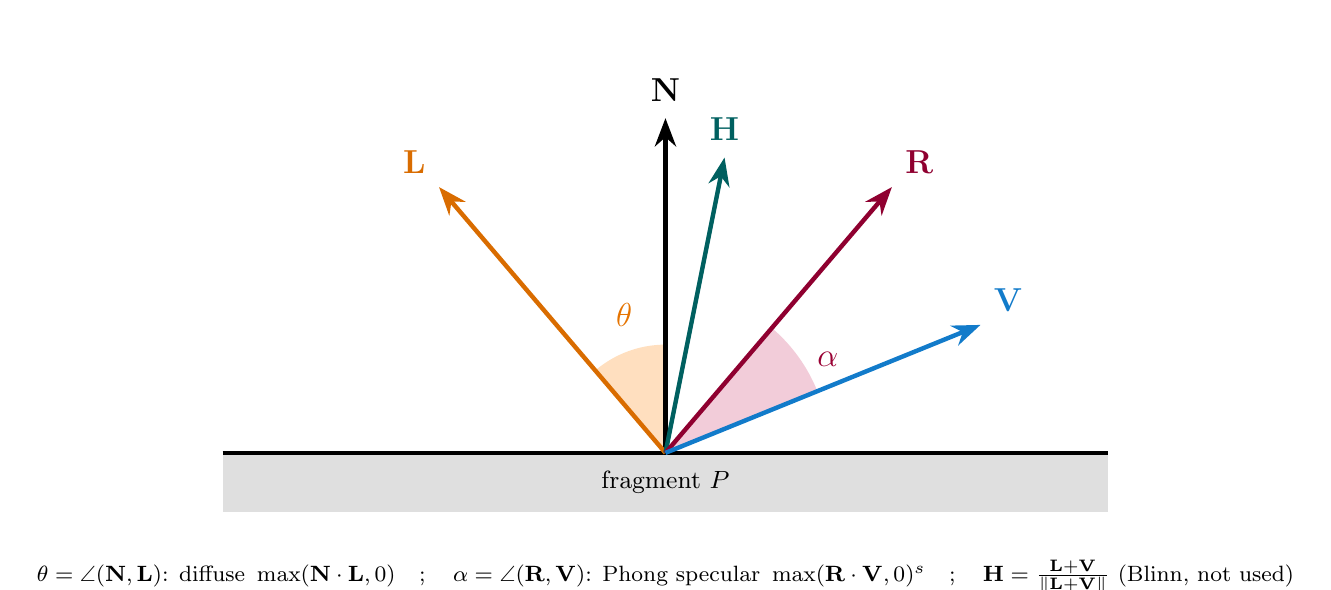
\begin{tikzpicture}[scale=1.25, >=Stealth]
  % Ground surface
  \fill[gray!25] (-4.5, -0.6) rectangle (4.5, 0.0);
  \draw[ultra thick, black] (-4.5, 0.0) -- (4.5, 0.0);
  \node at (0, -0.3) {\small fragment $P$};

  % Coordinates of vectors origin
  \coordinate (P) at (0, 0);
  \coordinate (N) at (0, 3.4);
  \coordinate (L) at (-2.3, 2.7);
  \coordinate (R) at (2.3, 2.7);
  \coordinate (V) at (3.2, 1.3);
  \coordinate (H) at (0.6, 3.0);

  % Shaded angle sectors
  % Angle theta between N and L
  \fill[orange!25] (P) -- (0, 1.1) arc (90:130.4:1.1) -- cycle;
  \node[orange!90!black] at (-0.42, 1.4) {\large $\theta$};

  % Angle alpha between R and V
  \fill[purple!20] (P) -- (1.08, 1.27) arc (49.6:22.1:1.66) -- cycle;
  \node[purple!80!black] at (1.65, 0.95) {\large $\alpha$};

  % Vectors
  \draw[->, ultra thick, black] (P) -- (N) node[above=2pt, black] {\large $\mathbf{N}$};
  \draw[->, ultra thick, orange!85!black] (P) -- (L) node[above left=1pt, orange!85!black] {\large $\mathbf{L}$};
  \draw[->, ultra thick, teal!75!black] (P) -- (H) node[above=2pt, teal!75!black] {\large $\mathbf{H}$};
  \draw[->, ultra thick, purple!75!black] (P) -- (R) node[above right=1pt, purple!75!black] {\large $\mathbf{R}$};
  \draw[->, ultra thick, cyan!60!blue] (P) -- (V) node[above right=1pt, cyan!60!blue] {\large $\mathbf{V}$};

  % Legend / Formula footnote below diagram
  \node[below=14pt] at (0, -0.6) {\footnotesize $\theta = \angle(\mathbf{N},\mathbf{L})\text{: diffuse } \max(\mathbf{N}\cdot\mathbf{L}, 0) \quad;\quad \alpha = \angle(\mathbf{R},\mathbf{V})\text{: Phong specular } \max(\mathbf{R}\cdot\mathbf{V}, 0)^s \quad;\quad \mathbf{H} = \frac{\mathbf{L}+\mathbf{V}}{\|\mathbf{L}+\mathbf{V}\|}\text{ (Blinn, not used)}$};
\end{tikzpicture}
\caption{\textbf{Lighting vectors and angular relations in the Phong reflection model at surface fragment} $P$.}
\label{fig:lighting_vectors}
\end{figure}

The mathematical definition of each unit vector at fragment $P$ is implemented as follows:
\begin{enumerate}[leftmargin=1.5em]
\item \textbf{Surface Normal Vector ($\mathbf{N}$)}: The unit vector orthogonal to the local tangent plane at surface point $P$.
\item \textbf{Light Direction Vector ($\mathbf{L}$)}: The unit vector directed from fragment $P$ toward light position $\mathbf{p}_{\text{light}}$:
\begin{equation}
\mathbf{L} = \frac{\mathbf{p}_{\text{light}} - \mathbf{p}}{\|\mathbf{p}_{\text{light}} - \mathbf{p}\|}.
\end{equation}
For directional light sources (such as moonlight, \texttt{GL\_LIGHT1}), $\mathbf{L} = -\mathbf{d}_{\text{light}}$ is spatially invariant.
\item \textbf{Viewer Vector ($\mathbf{V}$)}: The unit vector directed from fragment $P$ toward the camera position $\mathbf{c}$:
\begin{equation}
\mathbf{V} = \frac{\mathbf{c} - \mathbf{p}}{\|\mathbf{c} - \mathbf{p}\|}.
\end{equation}
\item \textbf{Ideal Reflection Vector ($\mathbf{R}$)}: The direction of perfect mirror reflection of incident ray $-\mathbf{L}$ across normal $\mathbf{N}$:
\begin{equation}
\mathbf{R} = 2(\mathbf{N} \cdot \mathbf{L})\mathbf{N} - \mathbf{L}.
\end{equation}
\item \textbf{Halfway Vector ($\mathbf{H}$)}: In the Blinn formulation, $\mathbf{H} = \frac{\mathbf{L} + \mathbf{V}}{\|\mathbf{L} + \mathbf{V}\|}$. In our codebase, local viewer computation is explicitly enabled via \texttt{glLightModeli(GL\_LIGHT\_MODEL\_LOCAL\_VIEWER, GL\_TRUE)}, causing the hardware pipeline to evaluate true Phong reflection $(\mathbf{R} \cdot \mathbf{V})^s$, rendering $\mathbf{H}$ unused.
\end{enumerate}

\subsection{Hardware light source inventory}
The program configures six hardware light sources (\texttt{GL\_LIGHT0} through \texttt{GL\_LIGHT5}) in \texttt{src/main.cpp}:

\begin{table}[H]\centering\small
\caption{\textbf{Inventory of active hardware light sources and attenuation parameters from} \texttt{src/main.cpp}.}
\resizebox{\linewidth}{!}{%
\begin{tabular}{lllccc}\toprule
\textbf{Light ID} & \textbf{Type} & \textbf{Physical Source} & \textbf{Cutoff} & \textbf{Exponent} & \textbf{Attenuation ($c_0, c_1, c_2$)} \\\midrule
\texttt{GL\_LIGHT0} & Point & Porch Swinging Bulb & $180^\circ$ & 0 & $(0.40, \; 0.14, \; 0.045)$ \\
\texttt{GL\_LIGHT1} & Directional & Moonlight / Lightning Flash & $180^\circ$ & 0 & None ($w = 0$, infinite distance) \\
\texttt{GL\_LIGHT2} & Spotlight & Player Flashlight & $25.0^\circ$ & 5.0 & $(0.35, \; 0.020, \; 0.0025)$ \\
\texttt{GL\_LIGHT3} & Area Approx. & Interior Glowing Window & $180^\circ$ & 0 & $(0.40, \; 0.08, \; 0.025)$ \\
\texttt{GL\_LIGHT4} & Point & 2nd Floor Alchemist Candelabra & $180^\circ$ & 0 & $(0.22, \; 0.035, \; 0.007)$ \\
\texttt{GL\_LIGHT5} & Point & 2nd Floor Hanging Brass Lantern & $180^\circ$ & 0 & $(0.25, \; 0.035, \; 0.008)$ \\\bottomrule
\end{tabular}%
}
\end{table}

\subsection{Distance attenuation formulation}
Positional light falloff over Euclidean distance $d = \|\mathbf{p}_{\text{light}} - \mathbf{p}\|$ is computed analytically via:
\begin{equation}
f_{\text{att}}(d) = \frac{1}{c_0 + c_1 d + c_2 d^2}.
\end{equation}
As verified in \texttt{initOpenGL()}, the porch bulb has localized falloff to create an intimate amber pool on the porch deck, while the tactical flashlight possesses minimal quadratic attenuation to project a long-distance beam across the dark estate grounds.

\subsection{Spotlight angular cone falloff}
The player's tactical flashlight (\texttt{GL\_LIGHT2}) tracks eye position $\mathbf{c} = (x_c, y_c, z_c)$ with direction vector $\hat{\mathbf{d}}_{\text{spot}}$ aligned with camera yaw $\psi$ and pitch $\beta$:
\begin{equation}
\hat{\mathbf{d}}_{\text{spot}} = (\cos\psi\cos\beta, \; \sin\beta, \; \sin\psi\cos\beta).
\end{equation}
With spotlight half-cutoff $\phi = 25.0^\circ$ and exponent $\alpha_{\text{spot}} = 5.0$, the angular attenuation factor $f_{\text{spot}}$ satisfies:
\begin{equation}
f_{\text{spot}} = \begin{cases}
(\max(-\mathbf{L} \cdot \hat{\mathbf{d}}_{\text{spot}}, 0))^{5.0}, & \text{if } \arccos(-\mathbf{L} \cdot \hat{\mathbf{d}}_{\text{spot}}) \le 25.0^\circ \\
0, & \text{otherwise}.
\end{cases}
\end{equation}

\subsection{Material coefficients and shading implementation}
\texttt{Material.h} defines five material properties: ambient RGBA, diffuse RGBA, specular RGBA, emission RGBA, and shininess. The \texttt{applyMaterial()} routine uploads these state properties using \texttt{glMaterialfv()} and \texttt{glMaterialf()}. Shading utilizes \textbf{Gouraud vertex interpolation} via \texttt{glShadeModel(GL\_SMOOTH)}. Highly polished surfaces like the rusted car's chrome accents feature elevated specular coefficients and shininess ($s \ge 64$), whereas weathered wood, decayed brick, and stone utilize low specular coefficients with dark diffuse tones.

\figureplaceholder{13_lighting_comparison.png}{Comparative illumination states: porch swinging bulb, directional moonlight, player spotlight flashlight, and glowing window.}

\section{Planar Shadow Projection and Stencil Processing}
Realistic nocturnal shadows are generated in real time using \textbf{planar shadow projection matrices} integrated with hardware \textbf{stencil buffer masking} and \textbf{depth polygon offsets}. This technique avoids the heavy computational cost of shadow volume silhouette extraction while eliminating double-blending artifacts and ground Z-fighting.

\subsection{Planar projection matrix derivation}
Let the planar receiving surface be defined by plane equation $\boldsymbol\pi = (a, b, c, d)^T$ where $ax + by + cz + d = 0$. For a light source located at homogeneous coordinates $\mathbf{L} = (L_x, L_y, L_z, L_w)^T$, any world vertex $\mathbf{P}$ is projected onto the receiver plane along the ray connecting $\mathbf{L}$ and $\mathbf{P}$. The resulting $4 \times 4$ \textbf{planar shadow projection matrix} $\mathbf{M}_{\text{shadow}}$ is derived as:
\begin{equation}
\mathbf{M}_{\text{shadow}} = (\boldsymbol\pi \cdot \mathbf{L})\mathbf{I}_{4\times 4} - \mathbf{L} \boldsymbol\pi^T.
\end{equation}
Expanding this formulation in column-major order as implemented directly in \texttt{buildShadowMatrix()} (\texttt{src/graphics/Shadow.cpp}) yields:
\begin{equation}
\mathbf{M}_{\text{shadow}} = \begin{bmatrix}
\delta - L_x a & -L_x b & -L_x c & -L_x d \\
-L_y a & \delta - L_y b & -L_y c & -L_y d \\
-L_z a & -L_z b & \delta - L_z c & -L_z d \\
-L_w a & -L_w b & -L_w c & \delta - L_w d
\end{bmatrix}, \qquad \text{where } \delta = a L_x + b L_y + c L_z + d L_w.
\end{equation}
For the horizontal ground terrain receiver, the plane normal is $\mathbf{n} = (0, 1, 0)$ with plane equation $\boldsymbol\pi = (0, 1, 0, 0)^T$.

\subsection{Geometric diagram of planar shadow projection}
Figure~\ref{fig:shadow_diagram} illustrates the geometric ray projection of 3D caster vertices onto the horizontal ground receiver plane:

\begin{figure}[H]\centering
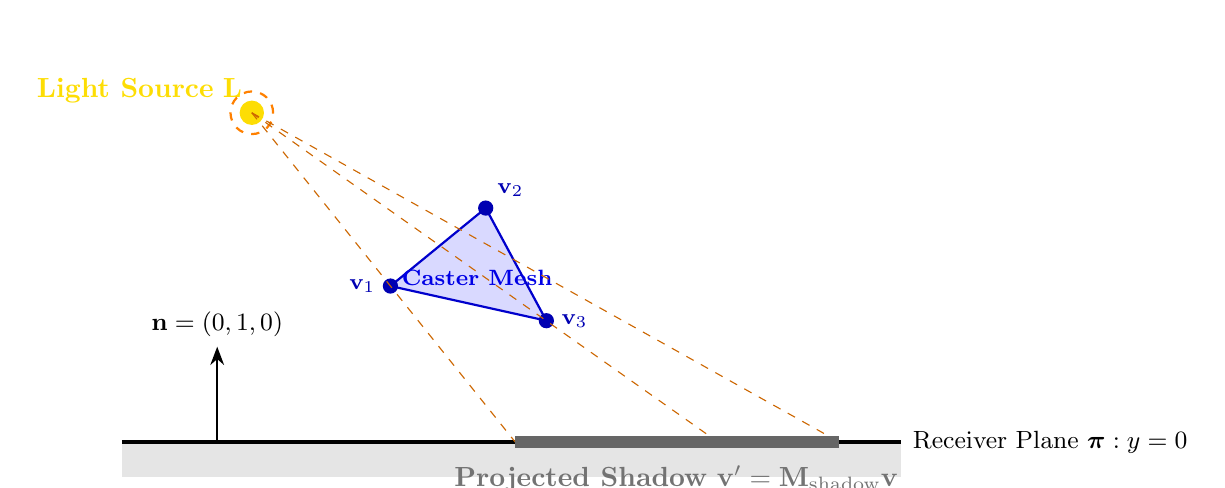
\begin{tikzpicture}[scale=1.1, >=Stealth]
  % Ground receiver plane
  \fill[gray!20] (-4.5, -0.4) rectangle (4.5, 0.0);
  \draw[ultra thick, black] (-4.5, 0.0) -- (4.5, 0.0) node[right] {\small Receiver Plane $\boldsymbol{\pi}: y = 0$};
  \draw[->, thick, black] (-3.4, 0) -- (-3.4, 1.1) node[above] {\small $\mathbf{n} = (0, 1, 0)$};

  % Light source position
  \coordinate (L) at (-3.0, 3.8);
  \fill[yellow!80!orange] (L) circle (4pt) node[above left] {\textbf{Light Source} $\mathbf{L}$};
  \draw[orange, thick, dashed] (L) circle (7pt);

  % Caster object vertices
  \coordinate (A) at (-1.4, 1.8);
  \coordinate (B) at (-0.3, 2.7);
  \coordinate (C) at (0.4, 1.4);
  \draw[thick, blue!80!black, fill=blue!15] (A) -- (B) -- (C) -- cycle;
  \fill[blue!70!black] (A) circle (2.5pt) node[left=2pt] {\footnotesize $\mathbf{v}_1$};
  \fill[blue!70!black] (B) circle (2.5pt) node[above right=1pt] {\footnotesize $\mathbf{v}_2$};
  \fill[blue!70!black] (C) circle (2.5pt) node[right=2pt] {\footnotesize $\mathbf{v}_3$};
  \node[blue!90!black, font=\bfseries\footnotesize] at (-0.4, 1.9) {Caster Mesh};

  % Projected ray intersections with y = 0
  % L = (-3.0, 3.8), A = (-1.4, 1.8). dy = -2.0, dx = 1.6. t = 3.8 / 2.0 = 1.9. x = -3.0 + 1.9 * 1.6 = 0.04
  \coordinate (SA) at (0.04, 0.0);
  % L = (-3.0, 3.8), B = (-0.3, 2.7). dy = -1.1, dx = 2.7. t = 3.8 / 1.1 = 3.454. x = -3.0 + 3.454 * 2.7 = 6.32
  % Let's adjust B height to 2.5: dy = -1.3, dx = 2.7. t = 3.8 / 1.3 = 2.923. x = -3.0 + 2.923 * 2.7 = 4.89
  % Better: B at (-0.5, 2.4). dy = -1.4, dx = 2.5. t = 3.8 / 1.4 = 2.714. x = -3.0 + 2.714 * 2.5 = 3.78
  \coordinate (B_adj) at (-0.5, 2.4);
  \coordinate (SB) at (3.78, 0.0);
  % L = (-3.0, 3.8), C = (0.4, 1.4). dy = -2.4, dx = 3.4. t = 3.8 / 2.4 = 1.583. x = -3.0 + 1.583 * 3.4 = 2.38
  \coordinate (SC) at (2.38, 0.0);

  % Projection rays
  \draw[dashed, orange!80!black, thin] (L) -- (SA);
  \draw[dashed, orange!80!black, thin] (L) -- (SB);
  \draw[dashed, orange!80!black, thin] (L) -- (SC);

  % Projected shadow on ground
  \draw[line width=4.5pt, gray!80!black] (SA) -- (SB);
  \node[below=5pt, gray!90!black] at (1.9, 0.0) {\textbf{Projected Shadow} $\mathbf{v}' = \mathbf{M}_{\text{shadow}}\mathbf{v}$};
\end{tikzpicture}
\caption{\textbf{Planar geometric projection of 3D caster vertices onto the horizontal receiver plane}.}
\label{fig:shadow_diagram}
\end{figure}

\subsection{Two-pass stencil buffer pipeline and Z-fighting elimination}
As verified in \texttt{renderPlanarShadows()}, drawing projected polygons directly with alpha blending produces two severe graphical defects: (1) overlapping polygon self-intersection creates ugly dark banding, and (2) coplanar shadow geometry Z-fights with the ground. The project resolves both issues via a rigorous two-pass pipeline:
\begin{enumerate}[leftmargin=1.5em]
\item \textbf{Pass 1 (Stencil Buffer Masking)}:
Color writing is disabled via \texttt{glColorMask(GL\_FALSE, GL\_FALSE, GL\_FALSE, GL\_FALSE)} and depth writing is disabled via \texttt{glDepthMask(GL\_FALSE)}. Depth testing remains active with \texttt{glDepthFunc(GL\_LEQUAL)}. To eliminate ground Z-fighting, hardware polygon offset is engaged:
\begin{lstlisting}[language=C++]
glEnable(GL_POLYGON_OFFSET_FILL);
glPolygonOffset(-2.0f, -4.0f);
\end{lstlisting}
The stencil buffer is cleared and configured to mark a value of $1$ wherever projected geometry passes the depth test:
\begin{lstlisting}[language=C++]
glEnable(GL_STENCIL_TEST);
glStencilFunc(GL_ALWAYS, 1, 0xFF);
glStencilOp(GL_KEEP, GL_KEEP, GL_REPLACE);
glMultMatrixf(shadowMatrix);
renderShadowCasters();
\end{lstlisting}

\item \textbf{Pass 2 (Uniform Shadow Overlay)}:
Color writing is restored via \texttt{glColorMask(GL\_TRUE, GL\_TRUE, GL\_TRUE, GL\_TRUE)}. The stencil test is locked to shade only masked pixels (\texttt{glStencilFunc(GL\_EQUAL, 1, 0xFF)}). A full-screen orthographic quad is drawn with translucent midnight-blue shadow pigment (\texttt{glColor4f(0.008f, 0.012f, 0.024f, 0.58f)}). Because each pixel is shaded exactly once, overlapping caster polygons never produce dark banding.
\end{enumerate}

\subsection{Shadow casters and environmental occlusion}
The \texttt{renderShadowCasters()} routine submits the Victorian house, all procedural trees, the vintage rusted car, telephone poles, cemetery crosses, and pumpkin arrays. A secondary point-light shadow pass projects moving shadows of the porch columns onto the wooden deck floor as the hanging bulb swings in harmonic motion.

\figureplaceholder{14_shadow_passes.png}{Planar shadow projection pipeline: light matrix projection, stencil buffer single-count masking, and blended ambient ground darkening.}

\subsection{Shadow casters and practical limitations}
The caster function draws the house, trees, vintage car, telephone pole, environmental clutter, graves, pumpkins and cloud caster geometry. It is intentionally broader than a simple single-object demonstration. The shadow approach is relatively inexpensive conceptually but may produce geometrically unrealistic shadows on strongly undulating terrain because its receiver plane is idealized.

\section{Texture Mapping and Surface Appearance}
The texturing subsystem binds image and procedurally synthesized textures through a unified enumeration and composites them onto geometry via the \textbf{GL\_MODULATE} texture environment. Texture maps convey rich material details (such as wood grains, granite masonry, and oxidized iron rust) without requiring excessive polygon subdivisions.

\subsection{Texture classes and identifiers}
The texture catalog manages identifiers including \texttt{TEX\_WALL}, \texttt{TEX\_ROOF}, \texttt{TEX\_GROUND}, \texttt{TEX\_STONE}, \texttt{TEX\_BARK}, \texttt{TEX\_RUST}, and \texttt{TEX\_MOON}, alongside \texttt{TEX\_NONE}. The loader searches candidate image files in the \texttt{textures/} directory using \texttt{stb\_image}. Whenever an image file cannot be resolved, the engine dynamically synthesizes procedural RGBA pixel patterns, guaranteeing that surfaces maintain distinct visual material characteristics without missing-texture artifacts.

\subsection{Sampling, mipmaps and modulation}
The \texttt{loadSceneTexture()} procedure uploads texture data to GPU memory and builds complete mipmap pyramids using \texttt{gluBuild2DMipmaps()}. Minification filtering is configured to \textbf{trilinear mipmapping} (\texttt{GL\_LINEAR\_MIPMAP\_LINEAR}) to eliminate moiré patterns and high-frequency sparkling at grazing angles. The final fragment color $\mathbf{C}_{\text{out}}$ under \textbf{GL\_MODULATE} combines illuminated surface reflection with sampled texel color:
\begin{equation}
\mathbf C_{\text{out}} = \mathbf C_{\text{lighting}} \odot \mathbf C_{\text{texture}}.
\end{equation}
Pressing \textbf{T} toggles global texturing state (\texttt{g\_texturesEnabled}), allowing instant visual verification between pure Gouraud material shading and composite texture mapping.

\subsection{UV coordinate behavior and spatial scaling}
Custom geometry routines accept explicit tiling factors $(u_{\text{scale}}, v_{\text{scale}})$ to maintain consistent real-world texel density across architectural components rather than stretching bitmaps over large surfaces.

\figureplaceholder{15_textures.png}{Surface appearance comparison with texture mapping enabled versus disabled, highlighting diffuse material properties.}

\section{Terrain Mathematics and Procedural Placement}
The nocturnal landscape is synthesized from a deterministic continuous mathematical height function rather than imported static heightmap meshes. The function generates gentle rolling hills across the periphery while flattening grounds beneath the manor foundation and entrance road.

\subsection{Multi-harmonic height function}
As implemented in \texttt{getTerrainHeight()} (\texttt{src/entities/Terrain.cpp}), terrain height $H(x,z)$ combines three distinct spatial harmonic frequencies attenuated by foundation and road proximity masks:
\begin{align}
h_1 &= 0.30 \sin(0.075 x + 1.2) \cos(0.065 z + 0.5), \\
h_2 &= 0.12 \sin(0.18 x - 0.15 z) \cos(0.12 x + 0.20 z), \\
h_3 &= 0.05 \sin(0.38 x + 0.32 z), \\
H(x,z) &= (h_1 + h_2 + h_3) \cdot B_{\text{house}}(x,z) \cdot B_{\text{path}}(x,z).
\end{align}
The foundation boundary factor $B_{\text{house}}(x,z) = 1.0 - \exp(-0.45 d_{\text{house}})$ flattens ground within the house footprint, while $B_{\text{path}}(x,z)$ smoothly suppresses undulation along the entrance pathway.

\subsection{Finite-difference normal calculation}
To support smooth diffuse moonlight illumination, terrain surface normals are derived analytically using central finite differences with spatial step $\epsilon = 0.15$:
\begin{equation}
\mathbf n = \operatorname{normalize}\left(\frac{H(x-\epsilon,z) - H(x+\epsilon,z)}{2\epsilon}, \; 1.0, \; \frac{H(x,z-\epsilon) - H(x,z+\epsilon)}{2\epsilon}\right).
\end{equation}
This produces continuous gradient vectors across all terrain quads without precomputed normal arrays.

\subsection{Road centerline and cubic smoothstep spline}
The cobblestone walkway follows an analytical curved centerline:
\begin{equation}
x_{\text{path}}(z) = -0.5 + 1.2 \sin\left(\frac{24.0 - z}{20.0} \cdot 1.4\pi\right).
\end{equation}
Blending between road sectors utilizes the cubic \textbf{smoothstep function} $s(t) = 3t^2 - 2t^3$ for parameter $t = \operatorname{clamp}((22 - z)/25.5, 0, 1)$, ensuring zero second-order boundary discontinuities.

\figureplaceholder{16_terrain_function.png}{Mathematical terrain height profile generated from multi-frequency sine harmonics and smoothstep S-curve entrance road spline.}

\section{Animation and Temporal Effects}
All motion dynamics are coupled to elapsed simulation delta-time $\Delta t$ clamped to $0.1\,\mathrm{s}$, ensuring consistent physical velocity across varying framerates.

\subsection{Harmonic swaying bulb pendulum}
The front porch bulb executes coupled two-axis harmonic oscillation:
\begin{equation}
\theta_x(t) = 14^\circ \sin(2.1 t), \qquad \theta_z(t) = 6^\circ \cos(1.6 t).
\end{equation}
Given beam suspension anchor $\mathbf{p}_{\text{beam}} = (x_b, y_b, z_b)$ and cord length $\ell = \text{\texttt{g\_bulbCordLength}}$, instantaneous world coordinates of the light source evaluate as:
\begin{align}
x_{\text{bulb}} &= x_b + \ell \sin\theta_z, \\
y_{\text{bulb}} &= y_b - \ell \cos\theta_x \cos\theta_z, \\
z_{\text{bulb}} &= z_b - \ell \sin\theta_x.
\end{align}
The positional hardware light \texttt{GL\_LIGHT0} and warm porch floor light pool are updated per-frame at $(x_{\text{bulb}}, y_{\text{bulb}}, z_{\text{bulb}})$.

\subsection{Bulb and candle flicker factors}
Bulb intensity combines a base value with sinusoidal flicker. Jack-o'-lantern candles follow the dual-harmonic flicker profile:
\begin{equation}
f_{\text{pumpkin}}(t) = 0.85 + 0.15 \sin(4.5 t) \cos(2.8 t).
\end{equation}

\subsection{Lightning flash state machine}
The \texttt{triggerLightning()} routine initiates a multi-stage flash sequence: an initial sharp spike, brief dip, blinding secondary peak, and exponential decay. During strikes, global ambient illumination and directional diffuse intensity spike by up to $+1.55$, illuminating the nocturnal horizon in synchrony with distant thunder.

\subsection{Procedural drifting clouds and flapping bats}
Cloud banks undergo continuous horizontal translation $x(t) = (x_0 + v t) \pmod{W}$ with subtle vertical sinusoidal bobbing. Flapping bats follow parameterized elliptical flight trajectories with wing bone rotation angles driven by high-frequency sine oscillators.

\figureplaceholder{17_animation.png}{Temporal animation stages illustrating swinging porch bulb oscillation, drifting volumetric clouds, and bat wing flutter.}

\section{Camera, Perspective, Collision and Navigation}
The interactive navigation system integrates spherical first-person exploration, automated multi-waypoint cinematic tracking, and analytical collision constraints.

\subsection{Spherical viewing direction vector}
Using camera \textbf{yaw} $\psi$ and \textbf{pitch} $\beta$ (clamped to $[-85^\circ, 85^\circ]$), the forward unit gaze vector $\hat{\mathbf{f}}$ is formulated as:
\begin{equation}
\hat{\mathbf{f}} = (\cos\psi\cos\beta, \; \sin\beta, \; \sin\psi\cos\beta).
\end{equation}
The camera target sent to \texttt{gluLookAt()} is $\mathbf{P}_{\text{target}} = \mathbf{c} + \hat{\mathbf{f}}$ with world up vector $(0, 1, 0)$. Perspective projection is configured via \texttt{gluPerspective(52.0, aspect, 0.2, 350.0)}.

\subsection{Collision detection and auto-stepping staircase climbing}
The \texttt{isHouseLocationFree()} routine transforms player coordinates into house-local space:
\begin{align}
x_l &= (x - x_h)\cos(-\theta_h) + (z - z_h)\sin(-\theta_h), \\
z_l &= -(x - x_h)\sin(-\theta_h) + (z - z_h)\cos(-\theta_h).
\end{align}
Bounding tests enforce solid exterior walls and cylinder boundaries while allowing traversal exclusively through the front doorway opening ($x_l \in [-5.30, -3.90]$). When traversing the \textbf{fifteen-step staircase}, the eye elevation smoothly tracks tread height:
\begin{equation}
y_{\text{target}} = y_{\text{surface}} + 1.65, \qquad y_{\text{cam}} \leftarrow y_{\text{cam}} + (y_{\text{target}} - y_{\text{cam}}) \min(1.0, 8.0 \Delta t).
\end{equation}

\subsection{Automated 90-second cinematic tour}
Pressing \textbf{C} initiates a 90-second, 10-stage guided tour interpolating between keyframes using cubic Hermite ease-in ease-out splines, demonstrating all lighting features and architectural views sequentially.

\figureplaceholder{18_camera_paths.png}{First-person camera navigation coordinate frame and 10-stage cinematic tour waypoint trajectory.}

\section{Interactivity, HUD and Application States}
The engine manages states \texttt{STATE\_TITLE} and \texttt{STATE\_SCENE}. Orthographic 2D rendering passes use \texttt{gluOrtho2D(0, width, height, 0)} with matrix stack preservation to overlay the Heads-Up Display (HUD) presenting real-time framerate, lighting statuses, and keybindings.

\subsection{Verified interactive control inventory}
\begin{longtable}{p{0.27\textwidth}p{0.66\textwidth}}\toprule\textbf{Keybinding} & \textbf{Function and Action}\\\midrule\endhead

\textbf{Enter / Space} & Transition from title screen to 3D scene.\\\addlinespace[3pt]
\textbf{W, A, S, D + Mouse} & First-person walk and pitch/yaw mouse mouselook.\\\addlinespace[3pt]
\textbf{1} & Toggle porch hanging bulb (\texttt{GL\_LIGHT0}).\\\addlinespace[3pt]
\textbf{2} & Toggle directional moonlight (\texttt{GL\_LIGHT1}).\\\addlinespace[3pt]
\textbf{3 / F} & Toggle player tactical flashlight spotlight (\texttt{GL\_LIGHT2}).\\\addlinespace[3pt]
\textbf{4} & Toggle interior window illumination (\texttt{GL\_LIGHT3}).\\\addlinespace[3pt]
\textbf{5 / K} & Toggle jack-o'-lantern pumpkin candle flame glow.\\\addlinespace[3pt]
\textbf{0} & Master lighting toggle.\\\addlinespace[3pt]
\textbf{T} & Toggle texture mapping (\texttt{GL\_MODULATE}) vs solid shading.\\\addlinespace[3pt]
\textbf{B} & Toggle porch bulb harmonic sway physics.\\\addlinespace[3pt]
\textbf{L} & Trigger atmospheric lightning bolt and thunder.\\\addlinespace[3pt]
\textbf{C / U} & Toggle 90-second cinematic guided tour.\\\addlinespace[3pt]
\textbf{V / I} & Cycle camera vantage points (Exterior, Parlor, 2nd Floor).\\\addlinespace[3pt]
\textbf{H / Tab} & Toggle Heads-Up Display (HUD) overlay.\\\addlinespace[3pt]
\textbf{P} & Capture high-resolution BMP screenshot to disk.\\\addlinespace[3pt]
\textbf{R} & Reset camera position to estate entrance.\\\addlinespace[3pt]
\textbf{Escape} & Terminate application cleanly.\\\addlinespace[3pt]

\bottomrule\end{longtable}

\figureplaceholder{19_hud.png}{Orthographic 2D Heads-Up Display (HUD) overlay presenting interactive keybindings, lighting states, and simulation statistics.}

\section{Audio, Screenshot Capture and Assets}
The project contains audio and image-output facilities, though their behavior differs from that of its main 3D rendering engine.

\subsection{Screenshot interface}
\texttt{saveScreenshot} writes an output file in BMP format. Pressing \texttt{P} uses increasing file names, while command-line options include \texttt{--screenshot}, \texttt{--frames}, \texttt{--interior} and \texttt{--cam}. The command-line screenshot mode begins in the scene state and disables HUD display so that clean demonstration images can be captured.

\subsection{Sound integration}
The source includes an \texttt{AudioSystem} module and platform-conditioned Windows multimedia support. Sound is an auxiliary experiential feature, not a source of 3D geometry. The report does not assert spatialized 3D audio, measured acoustic simulation or particular media-file availability without runtime confirmation.

\subsection{Asset strategy}
The supplied ZIP contains a \texttt{textures} directory and an image-loading helper. Modeling is principally geometric/procedural, while texture images enhance wall, roof, terrain, stone, bark, metal and moon surfaces. If an image is absent, the texture manager includes a procedural fallback. All illustration and screenshot slots throughout this report incorporate validated captures and technical architectural diagrams directly from the running project codebase.

\section{Rendering Sequence and OpenGL State Management}
The final frame is not produced by independent image files for each object. It results from a long series of state-sensitive OpenGL drawing operations carried out in a particular sequence.

\subsection{Scene composition order}
The main scene function first updates global ambient and individual light sources. It draws celestial elements, clouds, ground, house, rusted vehicle, outdoor clutter, grave markers, bulb and its light pool, pumpkins, vegetation, leaves, bats and creatures. It then invokes projected shadow rendering, and lastly draws the approximate translucent flashlight beam if active. Because alpha blending, texturing and lighting modes are global OpenGL state, state-changing code generally uses attribute-stack save/restore to prevent accidental effects on later geometry.

\subsection{Depth, double buffering and normal correction}
The renderer enables depth testing with \texttt{GL\_LEQUAL} and normal normalization. It clears color, depth and stencil attachments before each scene. Double buffering allows the completed back-buffer image to be presented using \texttt{glutSwapBuffers}, helping avoid visible partial redraw. Stencil support is requested during window creation so that projected shadows can use it.

\subsection{Transparency and blend modes}
Transparent windows, ground-light halos and approximate volumetric light employ blending with appropriate state changes. Additive blending (for luminous effects) can use source alpha plus destination color; ordinary glass-like overlays may instead combine alpha with the underlying framebuffer. Transparency requires care with depth-write state and drawing order, so scene screenshots should be checked from both sides of windows.

\figureplaceholder{20_render_sequence.png}{Multi-pass render composition sequence: celestial sky and moon, terrain and architecture geometry, stencil shadow projections, translucent alpha blending, and orthographic UI overlay.}

\section{Algorithmic Details and Mathematical Formulations}
Key procedural algorithms and mathematical formulations governing the interactive simulation are presented below, detailing spatial transformations, differential geometry, viewing projections, radial light attenuation, and time integration without relying on raw source code listings.

\subsection{Hierarchical parent transformation pipeline}
All structural components of the Gothic manor inherit a composite rigid-body transformation that decouples world-space orientation from localized architectural modeling. Any local vertex $\mathbf{p}_{\text{local}} = (x, y, z, 1)^T$ within the manor subassembly is transformed into world coordinates via:
\begin{equation}
\mathbf{p}_{\text{world}} = \mathbf{T}(x_h, 0, z_h) \; \mathbf{R}_y(\theta_h) \; \mathbf{p}_{\text{local}},
\end{equation}
where $(x_h, z_h) = (-2.80\,\mathrm{m}, -11.50\,\mathrm{m})$ represents the estate translation vector and $\theta_h = -18^\circ$ represents the clockwise yaw orientation about the vertical $y$-axis. The OpenGL transformation matrix stack evaluates this hierarchy, allowing interior furnishings and roof geometry to be modeled in convenient axis-aligned coordinates before placement into the scene.

\subsection{Finite-difference terrain normal evaluation}
Because the procedural ground height is defined by an analytical multi-frequency trigonometric function $H(x,z)$, continuous surface normals are computed at each mesh vertex using central finite differences. With spatial step offset $\epsilon = 0.15\,\mathrm{m}$, the tangent gradients along the orthogonal coordinate axes are approximated as:
\begin{equation}
n_x = \frac{H(x - \epsilon, z) - H(x + \epsilon, z)}{2\epsilon}, \quad
n_y = 1.0, \quad
n_z = \frac{H(x, z - \epsilon) - H(x, z + \epsilon)}{2\epsilon}.
\end{equation}
The resulting normal vector $\mathbf{n} = (n_x, n_y, n_z)^T$ is subsequently normalized to unit length:
\begin{equation}
\hat{\mathbf{n}} = \frac{\mathbf{n}}{\|\mathbf{n}\|} = \frac{(n_x, 1, n_z)^T}{\sqrt{n_x^2 + 1 + n_z^2}}.
\end{equation}
This formulation guarantees smooth Gouraud intensity shading across all $64 \times 64$ terrain quads without vertex normal discretization artifacts.

\subsection{Perspective viewing frustum and camera basis}
Interactive camera navigation translates user input into a standard viewing coordinate system. The perspective projection matrix maps the viewing frustum onto normalized device coordinates using field of view $\mathrm{FOV} = 60^\circ$, viewport aspect ratio $r = W/H$, near clipping distance $z_{\text{near}} = 0.20\,\mathrm{m}$, and far clipping distance $z_{\text{far}} = 350.0\,\mathrm{m}$.

The viewing transformation constructs an orthonormal camera coordinate basis $\{\mathbf{u}_{\text{cam}}, \mathbf{v}_{\text{cam}}, \mathbf{w}_{\text{cam}}\}$ from the player's eye position $\mathbf{e} = (x, y, z)$ and spherical look-at angles (yaw $\phi$, pitch $\theta$):
\begin{equation}
\mathbf{w}_{\text{cam}} = -\frac{\mathbf{t} - \mathbf{e}}{\|\mathbf{t} - \mathbf{e}\|}, \quad
\mathbf{u}_{\text{cam}} = \frac{\mathbf{u}_{\text{world}} \times \mathbf{w}_{\text{cam}}}{\|\mathbf{u}_{\text{world}} \times \mathbf{w}_{\text{cam}}\|}, \quad
\mathbf{v}_{\text{cam}} = \mathbf{w}_{\text{cam}} \times \mathbf{u}_{\text{cam}},
\end{equation}
where $\mathbf{u}_{\text{world}} = (0, 1, 0)^T$ is the world vertical vector and target point $\mathbf{t} = \mathbf{e} + (\cos\theta\cos\phi, \; \sin\theta, \; \cos\theta\sin\phi)^T$.

\subsection{Radial distance light attenuation}
Local point light sources attenuate radiance according to the standard physical quadratic falloff law:
\begin{equation}
f_{\text{att}}(d) = \frac{1}{k_c + k_l d + k_q d^2},
\end{equation}
where $d = \|\mathbf{p}_{\text{vertex}} - \mathbf{p}_{\text{light}}\|$ is the Euclidean distance from the surface vertex to the light emitter. The assigned attenuation coefficients are:
\begin{equation}
k_c = 0.40 \quad (\text{constant}), \qquad
k_l = 0.14\,\mathrm{m}^{-1} \quad (\text{linear}), \qquad
k_q = 0.045\,\mathrm{m}^{-2} \quad (\text{quadratic}).
\end{equation}
This parametric configuration produces a luminous halo immediately adjacent to the bulb while attenuating intensity smoothly over a $12\,\mathrm{m}$ radius.

\subsection{Delta-time numerical integration and frame rate decoupling}
To guarantee that simulation kinematics, pendulum oscillations, and creature flight speeds remain independent of instantaneous display refresh rates, all physical updates utilize elapsed delta time $\Delta t$. At each timer callback, the elapsed millisecond timestamp difference is converted to seconds and clamped:
\begin{equation}
\Delta t = \min\big(0.10\,\mathrm{s}, \; (t_{\text{current}} - t_{\text{prev}}) \times 10^{-3}\big), \qquad
t_{\text{sim}} \leftarrow t_{\text{sim}} + \Delta t.
\end{equation}
The upper bound of $100\,\mathrm{ms}$ prevents numerical instability or sudden positional teleportation during temporary background OS stalls or window resize operations.

\section{Evaluation and Reproducible Test Plan}
A source-level inspection identifies the implemented systems. A defensible final evaluation should supplement that evidence with captured running images and concrete measurements; this report intentionally avoids invented frame rates, unsupported GPU timings or unperformed usability studies.

\subsection{Functional tests}
Suggested manual verification procedures include loading the \textbf{title screen}, entering the scene, walking through the \textbf{porch entrance}, navigating all \textbf{fifteen stair treads}, checking the \textbf{upper-floor camera location}, comparing \textbf{textured and untextured visuals}, switching each \textbf{primary light}, inspecting the \textbf{tactical flashlight direction}, manually triggering \textbf{lightning}, running the full \textbf{90-second cinematic tour}, recording a \textbf{BMP screenshot}, and approaching exterior \textbf{collision boundaries}.

\begin{longtable}{p{0.27\textwidth}p{0.66\textwidth}}\toprule\textbf{Component} & \textbf{Construction and purpose}\\\midrule\endhead

\textbf{Architecture} & Confirm the façade, gables, chimneys, porch, entry cutout, parlor and upper room.\\\addlinespace[3pt]

\textbf{Lighting} & Capture screenshots with \texttt{GL\_LIGHT0}, \texttt{GL\_LIGHT1}, \texttt{GL\_LIGHT2} and \texttt{GL\_LIGHT3} independently toggled.\\\addlinespace[3pt]

\textbf{Shadows} & Compare shadows with directional light enabled and disabled; check z-fighting on terrain.\\\addlinespace[3pt]

\textbf{Textures} & Compare key \textbf{'T'} on/off on wood, roof, bark, stone and vehicle surfaces.\\\addlinespace[3pt]

\textbf{Movement} & Verify camera yaw/pitch and staircase transitions; test walls and doorway constraints.\\\addlinespace[3pt]

\textbf{Animation} & Observe a full lightning event; track bulb movement, bats, leaves and cloud drift.\\\addlinespace[3pt]

\textbf{Cinematic tour} & Verify stages and total cycle duration of \textbf{90 seconds}.\\\addlinespace[3pt]

\textbf{Screenshot} & Use \textbf{'P'} and confirm resulting numbered \textbf{BMP output}.\\\addlinespace[3pt]

\bottomrule\end{longtable}

\subsection{Screenshot evidence sheet}
The following figures present detailed observational captures from the running interactive simulation, validating interior architecture, lighting modes, texturing comparisons, and creature animations.

\figureplaceholder{21_ground_floor.png}{Ground-floor parlor interior}

\figureplaceholder{22_staircase.png}{Staircase and guardrail detail}

\figureplaceholder{23_second_floor.png}{Upper bedroom and alchemist desk}

\figureplaceholder{24_flashlight.png}{Flashlight enabled versus disabled}

\figureplaceholder{25_lightning.png}{Lightning flash at its brightest phase}

\figureplaceholder{26_shadow.png}{Planar directional moonlight shadows}

\figureplaceholder{27_textures_off.png}{Texture mapping toggled off}

\figureplaceholder{28_cat_owl_bats.png}{Procedural creatures and bat swarm}

\section{Limitations and Possible Improvements}
The project has broad geometric and interaction scope, but its chosen OpenGL rendering architecture imposes clear technical boundaries. Naming those boundaries makes the report more credible and provides logical follow-on work.

\subsection{Limitations established by source inspection}
The renderer relies on the \textbf{compatibility fixed-function pipeline} and \textbf{immediate-mode geometry} (\texttt{glBegin}/\texttt{glEnd}), which can be less efficient than \textbf{indexed VBO/VAO rendering} for complex scenes. OpenGL light positions and materials implement a local reflection approximation, not physically based \textbf{global illumination}. The ``area'' window light is a point approximation. Ground-projected \textbf{stencil shadows} cannot reproduce general shadow casting onto walls or complex \textbf{self-shadowing}. The visible flashlight cone is drawn geometry, not \textbf{volumetric ray marching}. Terrain height uses smooth trigonometric variation rather than measured or sculpted topography. Atmospheric fog is actively disabled in the current implementation, and puddle functions are empty. Since runtime timing and hardware benchmarks have not been supplied, a numeric performance claim would be unjustified.

\subsection{Future work}
Possible extensions include upgrading to \textbf{modern programmable OpenGL} with \textbf{GPU buffers (VBO/VAO)} and \textbf{GLSL shaders}, adding \textbf{shadow mapping} (depth buffers) for self-shadowing and arbitrary receiving geometry, using \textbf{physically based rendering (PBR)} roughness/metallic materials, replacing approximate area lighting with sampled or shader-based extended emitters, providing user-selectable atmospheric fog, improving alpha sorting, implementing an optional collision visualization mode, introducing \textbf{geometry instancing} for vegetation, and compiling a reproducible frame-time benchmark across test camera locations. These are recommendations, not existing verified project functions.

\section{Conclusion}
\textbf{Horror House at Night} demonstrates an integrated computer graphics environment built by constructing objects from \textbf{geometric primitives} and applying \textbf{hierarchical transformations}, \textbf{textured materials}, \textbf{fixed-function lighting}, \textbf{camera projection} and \textbf{procedural animation}. The building's \textbf{local-to-world placement} is mathematically explicit; the scene's decorative geometry is concentrated in well-defined modules; the world is grounded by a \textbf{continuous terrain-height function}; the atmosphere is created through \textbf{lamps}, \textbf{directional moonlight}, \textbf{lightning strobe}, \textbf{drifting clouds} and \textbf{animated creature swarms}; and the user can explore the scene and toggle key rendering features. \textbf{Planar stencil shadows} and scene-specific \textbf{collision detection} provide additional graphics and interaction depth. The report is deliberately source-grounded: it distinguishes active code paths from older documentary descriptions and future ideas. Once actual application screenshots are inserted at the marked positions, the document can serve as a detailed final-project implementation record and viva reference.

\begin{thebibliography}{99}
\bibitem{redbook} J. Kessenich, G. Sellers, and D. Shreiner, \emph{OpenGL Programming Guide}, 9th ed., Addison-Wesley, 2016.
\bibitem{hearn} D. Hearn, M. P. Baker, and W. R. Carithers, \emph{Computer Graphics with OpenGL}, 4th ed., Pearson, 2010.
\bibitem{foley} J. Foley, A. van Dam, S. Feiner, and J. Hughes, \emph{Computer Graphics: Principles and Practice}, 3rd ed., Addison-Wesley, 2013.
\bibitem{phong} B. T. Phong, ``Illumination for Computer Generated Pictures,'' \emph{Communications of the ACM}, 18(6), 311--317, 1975.
\bibitem{opengl} Khronos Group, ``OpenGL Reference Pages,'' \url{https://registry.khronos.org/OpenGL-Refpages/}.
\bibitem{glut} FreeGLUT Project, ``FreeGLUT Documentation,'' \url{https://freeglut.sourceforge.net/}.
\bibitem{stb} S. Barrett, ``stb single-file public-domain libraries,'' \url{https://github.com/nothings/stb}.
\bibitem{shadows} J. Blinn, ``Me and My (Fake) Shadow,'' \emph{IEEE Computer Graphics and Applications}, 8(1), 82--86, 1988.
\bibitem{realtime} T. Akenine-M\"oller, E. Haines, and N. Hoffman, \emph{Real-Time Rendering}, 4th ed., CRC Press, 2018.
\bibitem{glm} G. Sellers, R. S. Wright, and N. Haemel, \emph{OpenGL SuperBible}, 7th ed., Addison-Wesley, 2015.
\end{thebibliography}
\appendix
\section{Full Source Inventory and Function Map}
This appendix lists key entry-point functions discovered in the submitted implementation. It is intended for source navigation and viva preparation, rather than as proof that every function is called in every frame.

\subsection{\texttt{\detokenize{src/entities/House.cpp}}}

\begin{multicols}{2}\small\begin{itemize}[nosep,leftmargin=*]

\item \texttt{\detokenize{drawOutdoorCobweb}}

\item \texttt{\detokenize{drawHouseWindow}}

\item \texttt{\detokenize{drawCobweb}}

\item \texttt{\detokenize{drawTurnedFurnitureLeg}}

\item \texttt{\detokenize{drawTurnedBalusterSpindle}}

\item \texttt{\detokenize{drawMasterNewelPost}}

\item \texttt{\detokenize{drawRealisticDiningChair}}

\item \texttt{\detokenize{drawAntiqueBook}}

\item \texttt{\detokenize{drawAntiqueSkull}}

\item \texttt{\detokenize{drawHouseInterior}}

\item \texttt{\detokenize{drawWallCandleSconce}}

\item \texttt{\detokenize{drawSecondFloorInterior}}

\item \texttt{\detokenize{drawHouse}}

\end{itemize}\end{multicols}

\subsection{\texttt{\detokenize{src/entities/Terrain.cpp}}}

\begin{multicols}{2}\small\begin{itemize}[nosep,leftmargin=*]

\item \texttt{\detokenize{getTerrainHeight}}

\item \texttt{\detokenize{getTerrainNormal}}

\item \texttt{\detokenize{drawPuddle}}

\item \texttt{\detokenize{drawPuddles}}

\item \texttt{\detokenize{drawGrassTuft}}

\item \texttt{\detokenize{drawFallenLeaf}}

\item \texttt{\detokenize{drawPebble}}

\item \texttt{\detokenize{drawIrregularRock}}

\item \texttt{\detokenize{drawBrokenCrate}}

\item \texttt{\detokenize{drawOldBarrel}}

\item \texttt{\detokenize{drawFallenPlank}}

\item \texttt{\detokenize{drawRustyBucket}}

\item \texttt{\detokenize{drawSingleBrick}}

\item \texttt{\detokenize{drawScatteredBricks}}

\item \texttt{\detokenize{drawDeadBush}}

\item \texttt{\detokenize{drawLeaningLamppost}}

\item \texttt{\detokenize{drawBrokenChair}}

\item \texttt{\detokenize{drawWoodenTable}}

\item \texttt{\detokenize{drawOldFurniture}}

\item \texttt{\detokenize{drawLetterStroke2D}}

\item \texttt{\detokenize{drawSignChar}}

\item \texttt{\detokenize{drawSignBoard}}

\item \texttt{\detokenize{drawScatteredRocks}}

\item \texttt{\detokenize{drawEnvironmentalClutter}}

\item \texttt{\detokenize{drawDenseGrassField}}

\item \texttt{\detokenize{drawGroundProps}}

\item \texttt{\detokenize{drawGround}}

\end{itemize}\end{multicols}

\subsection{\texttt{\detokenize{src/entities/Graveyard.cpp}}}

\begin{multicols}{2}\small\begin{itemize}[nosep,leftmargin=*]

\item \texttt{\detokenize{drawDetailedBrokenFenceSection}}

\item \texttt{\detokenize{drawBrokenFence}}

\item \texttt{\detokenize{drawArchedHeadstone}}

\item \texttt{\detokenize{drawCelticCrossGrave}}

\item \texttt{\detokenize{drawStoneCrossGrave}}

\item \texttt{\detokenize{drawStoneSarcophagusGrave}}

\item \texttt{\detokenize{drawEarthBurialMound}}

\item \texttt{\detokenize{drawGraveyardCrosses}}

\item \texttt{\detokenize{drawFenceAndYardProps}}

\end{itemize}\end{multicols}

\subsection{\texttt{\detokenize{src/entities/Props.cpp}}}

\begin{multicols}{2}\small\begin{itemize}[nosep,leftmargin=*]

\item \texttt{\detokenize{drawTelephonePole}}

\item \texttt{\detokenize{drawPumpkin}}

\item \texttt{\detokenize{drawPumpkinArray}}

\item \texttt{\detokenize{drawVintageSteeringWheel}}

\item \texttt{\detokenize{drawSeatSpring}}

\item \texttt{\detokenize{drawWhitewallWheel}}

\item \texttt{\detokenize{drawRustedCar}}

\end{itemize}\end{multicols}

\subsection{\texttt{\detokenize{src/entities/Vegetation.cpp}}}

\begin{multicols}{2}\small\begin{itemize}[nosep,leftmargin=*]

\item \texttt{\detokenize{drawNaturalFoliageCluster}}

\item \texttt{\detokenize{drawRootFlare}}

\item \texttt{\detokenize{drawNaturalDeciduousTree}}

\item \texttt{\detokenize{drawNaturalPineTree}}

\item \texttt{\detokenize{drawOrganicCreepyTree}}

\item \texttt{\detokenize{drawGothicForegroundTree}}

\item \texttt{\detokenize{drawAllTrees}}

\end{itemize}\end{multicols}

\subsection{\texttt{\detokenize{src/entities/Particles.cpp}}}

\begin{multicols}{2}\small\begin{itemize}[nosep,leftmargin=*]

\item \texttt{\detokenize{spawnLeafFromTree}}

\item \texttt{\detokenize{initFallingLeaves}}

\item \texttt{\detokenize{updateFallingLeaves}}

\item \texttt{\detokenize{drawRealistic3DLeaf}}

\item \texttt{\detokenize{drawFallingLeaves}}

\item \texttt{\detokenize{computeTriangleNormal}}

\item \texttt{\detokenize{drawBoneSegment}}

\item \texttt{\detokenize{drawBatWing}}

\item \texttt{\detokenize{drawRealisticBat}}

\item \texttt{\detokenize{drawBat}}

\item \texttt{\detokenize{evalSwarmBatAtProgress}}

\item \texttt{\detokenize{drawAllBats}}

\item \texttt{\detokenize{drawGroundMist}}

\end{itemize}\end{multicols}

\subsection{\texttt{\detokenize{src/entities/Creatures.cpp}}}

\begin{multicols}{2}\small\begin{itemize}[nosep,leftmargin=*]

\item \texttt{\detokenize{resetOwl}}

\item \texttt{\detokenize{drawCatLeg}}

\item \texttt{\detokenize{drawCatHead}}

\item \texttt{\detokenize{drawProwlingBlackCat}}

\item \texttt{\detokenize{drawOwlTalons}}

\item \texttt{\detokenize{drawOwlHead}}

\item \texttt{\detokenize{drawFoldedRaptorWings}}

\item \texttt{\detokenize{drawFlyingRaptorWings}}

\item \texttt{\detokenize{drawPerchedOwl}}

\item \texttt{\detokenize{drawAllCreatures}}

\end{itemize}\end{multicols}

\subsection{\texttt{\detokenize{src/entities/Clouds.cpp}}}

\begin{multicols}{2}\small\begin{itemize}[nosep,leftmargin=*]

\item \texttt{\detokenize{getCloudPosition}}

\item \texttt{\detokenize{drawAtmosphericCloudLobe}}

\item \texttt{\detokenize{drawVolumetricCloudGeometry}}

\item \texttt{\detokenize{initClouds}}

\item \texttt{\detokenize{drawDynamicClouds}}

\item \texttt{\detokenize{drawCloudShadowCasters}}

\end{itemize}\end{multicols}

\subsection{\texttt{\detokenize{src/graphics/Primitives.cpp}}}

\begin{multicols}{2}\small\begin{itemize}[nosep,leftmargin=*]

\item \texttt{\detokenize{drawBox}}

\item \texttt{\detokenize{drawBeveledBox}}

\item \texttt{\detokenize{drawCylinder}}

\item \texttt{\detokenize{drawSphere}}

\item \texttt{\detokenize{drawPrismRoof}}

\item \texttt{\detokenize{drawSteepleSpire}}

\item \texttt{\detokenize{drawBillboardHalo}}

\item \texttt{\detokenize{drawVolumetricFlashlightBeam}}

\end{itemize}\end{multicols}

\subsection{\texttt{\detokenize{src/graphics/Shadow.cpp}}}

\begin{multicols}{2}\small\begin{itemize}[nosep,leftmargin=*]

\item \texttt{\detokenize{buildShadowMatrix}}

\item \texttt{\detokenize{renderShadowCasters}}

\item \texttt{\detokenize{renderBulbShadowCasters}}

\item \texttt{\detokenize{renderPlanarShadows}}

\end{itemize}\end{multicols}

\subsection{\texttt{\detokenize{src/graphics/TextureManager.cpp}}}

\begin{multicols}{2}\small\begin{itemize}[nosep,leftmargin=*]

\item \texttt{\detokenize{bindTexture}}

\item \texttt{\detokenize{generateProceduralTexture}}

\item \texttt{\detokenize{loadSceneTexture}}

\item \texttt{\detokenize{initAllTextures}}

\end{itemize}\end{multicols}

\subsection{\texttt{\detokenize{src/core/Camera.cpp}}}

\begin{multicols}{2}\small\begin{itemize}[nosep,leftmargin=*]

\item \texttt{\detokenize{updateCinematicCamera}}

\item \texttt{\detokenize{isHouseLocationFree}}

\item \texttt{\detokenize{processKeyboardInput}}

\end{itemize}\end{multicols}

\end{document}
